\documentclass[UTF8]{beamer}

\usepackage[backend=bibtex,sorting=none]{biblatex}
\addbibresource{reference.bib}
\setbeamerfont{footnote}{size=\tiny}

% \usepackage{fontspec}

% \usepackage[backref, colorlinks,
%     linkcolor=black,
%     citecolor=blue,
%     urlcolor=magenta
% ]{hyperref}

\usepackage{amsmath, amsfonts, amssymb, amsthm, extarrows, mathdots}

\usepackage{soul}

\usepackage{enumerate}

\usepackage{xcolor}

\usepackage{graphicx}

\usepackage{subfigure}

\usepackage{url}

\usepackage{bm}

\usepackage{multirow}

\usepackage{booktabs}

\usepackage{epstopdf}

\usepackage{epsfig}

\usepackage{listings}

\usepackage{longtable}

\usepackage{supertabular}

\usepackage{algorithm}

\usepackage{algorithmic}

\usepackage{changepage}

\usepackage{authblk}

% \lstset{
% 	basicstyle=\ttfamily,	% 基本样式
% 		keywordstyle=\color{blue}, % 关键词样式
% 		commentstyle=\color{gray!50!black!50},   	% 注释样式
% 		stringstyle=\rmfamily\slshape\color{red}, 	% 字符串样式
% 	backgroundcolor=\color{gray!5},     % 代码块背景颜色
% 	frame=leftline,						% 代码框形状
% 	framerule=12pt,%
% 		rulecolor=\color{gray!90},      % 代码框颜色
% 	numbers=left,				% 左侧显示行号往左靠, 还可以为right ,或none,即不加行号
% 		numberstyle=\footnotesize\itshape,	% 行号的样式
% 		firstnumber=1,
% 		stepnumber=1,                  	% 若设置为2,则显示行号为1,3,5
% 		numbersep=7pt,               	% 行号与代码之间的间距
% 	aboveskip=.25em, 			% 代码块边框
% 	showspaces=false,               	% 显示添加特定下划线的空格
% 	showstringspaces=false,         	% 不显示代码字符串中间的空格标记
% 	keepspaces=true, 					
% 	showtabs=false,                 	% 在字符串中显示制表符
% 	tabsize=2,                     		% 默认缩进2个字符
% 	captionpos=b,                   	% 将标题位置设置为底部
% 	flexiblecolumns=true, 			%
% 	breaklines=true,                	% 设置自动断行
% 	breakatwhitespace=false,        	% 设置自动中断是否只发生在空格处
% 	breakautoindent=true,			%
% 	breakindent=1em, 			%
% 	title=\lstname,				%
% 	escapeinside=``,  			% 在``里显示中文
% 	xleftmargin=1em,  xrightmargin=1em,     % 设定listing左右的空白
% 	aboveskip=1ex, belowskip=1ex,
% 	framextopmargin=1pt, framexbottommargin=1pt,
%         abovecaptionskip=-2pt,belowcaptionskip=3pt,
% 	% 设定中文冲突,断行,列模式,数学环境输入,listing数字的样式
% 	extendedchars=false, columns=flexible, mathescape=true,
% 	texcl=true,
% 	fontadjust
% }

% {
%     \theoremstyle{definition}
%     \newtheorem{axiom}{\indent 公理}
%     \newtheorem{theorem}{\indent 定理}[section]
%     \newtheorem{lemma}[theorem]{\indent 引理}
%     \newtheorem{proposition}[theorem]{\indent 命题}
%     \newtheorem{corollary}[theorem]{\indent 推论}
%     \newtheorem{definition}[theorem]{\indent 定义}
%     \newtheorem*{solution}{\indent 解}
%     \newtheorem{example}{\indent 例}[section]\theoremstyle{definition}
%     \newtheorem*{axiom*}{\indent 公理}
%     \newtheorem*{theorem*}{\indent 定理}
%     \newtheorem*{lemma*}{\indent 引理}
%     \newtheorem*{proposition*}{\indent 命题}
%     \newtheorem*{corollary*}{\indent 推论}
%     \newtheorem*{definition*}{\indent 定义}
%     \newtheorem*{example*}{\indent 例}
%     \renewcommand{\proofname}{\indent\bf 证明}
% }

\renewcommand{\proofname}{\indent\bf 证明}
\newcommand{\bra}[1]{\langle#1|}
\newcommand{\ket}[1]{|#1\rangle}
\newcommand{\inner}[2]{\langle#1|#2\rangle}
\newcommand{\tensor}{\otimes}
\newcommand{\xor}{\oplus}

\newcommand*{\dif}{\mathop{}\!\mathrm{d}}

% \usepackage{xpatch}
% \makeatletter
% \xpatchcmd{\@thm}{\thm@headpunct{.}}{\thm@headpunct{}}{}{}
% \makeatother


% {
%     \theoremstyle{plain}
%     \newtheorem*{think}{\indent 思考}
%     \newtheorem*{note}{\indent 注}
% }

% \def\equationautorefname{式}
% \def\footnoteautorefname{脚注}
% \def\itemautorefname{项}
% \def\figureautorefname{图}
% \def\tableautorefname{表}
% \def\partautorefname{篇}
% \def\appendixautorefname{附录}
% \def\chapterautorefname{章}
% \def\sectionautorefname{节}
% \def\subsectionautorefname{小节}
% \def\subsubsectionautorefname{小节}
% \def\paragraphautorefname{段落}
% \def\subparagraphautorefname{子段落}
% \def\FancyVerbLineautorefname{行}
% \def\theoremautorefname{定理}

% \setcounter{tocdepth}{2}
% \setcounter{secnumdepth}{3}


\usetheme{Warsaw}
\useoutertheme{miniframes}

\title{AI for System and System for AI}
\author[Conless Pan]{Conless Pan\inst{$\dagger$}}

\institute[SJTU]{
  \inst{$\dagger$}
  ACM Class 2022\\
  Shanghai Jiao Tong University
}

\date{\today}

\begin{document}

\begin{frame}[plain]
  \titlepage
\end{frame}

\begin{frame}
  \tableofcontents
\end{frame}

\section{Introduction}

\begin{frame}{The Rise of Machine Learning}
  \begin{center} 
    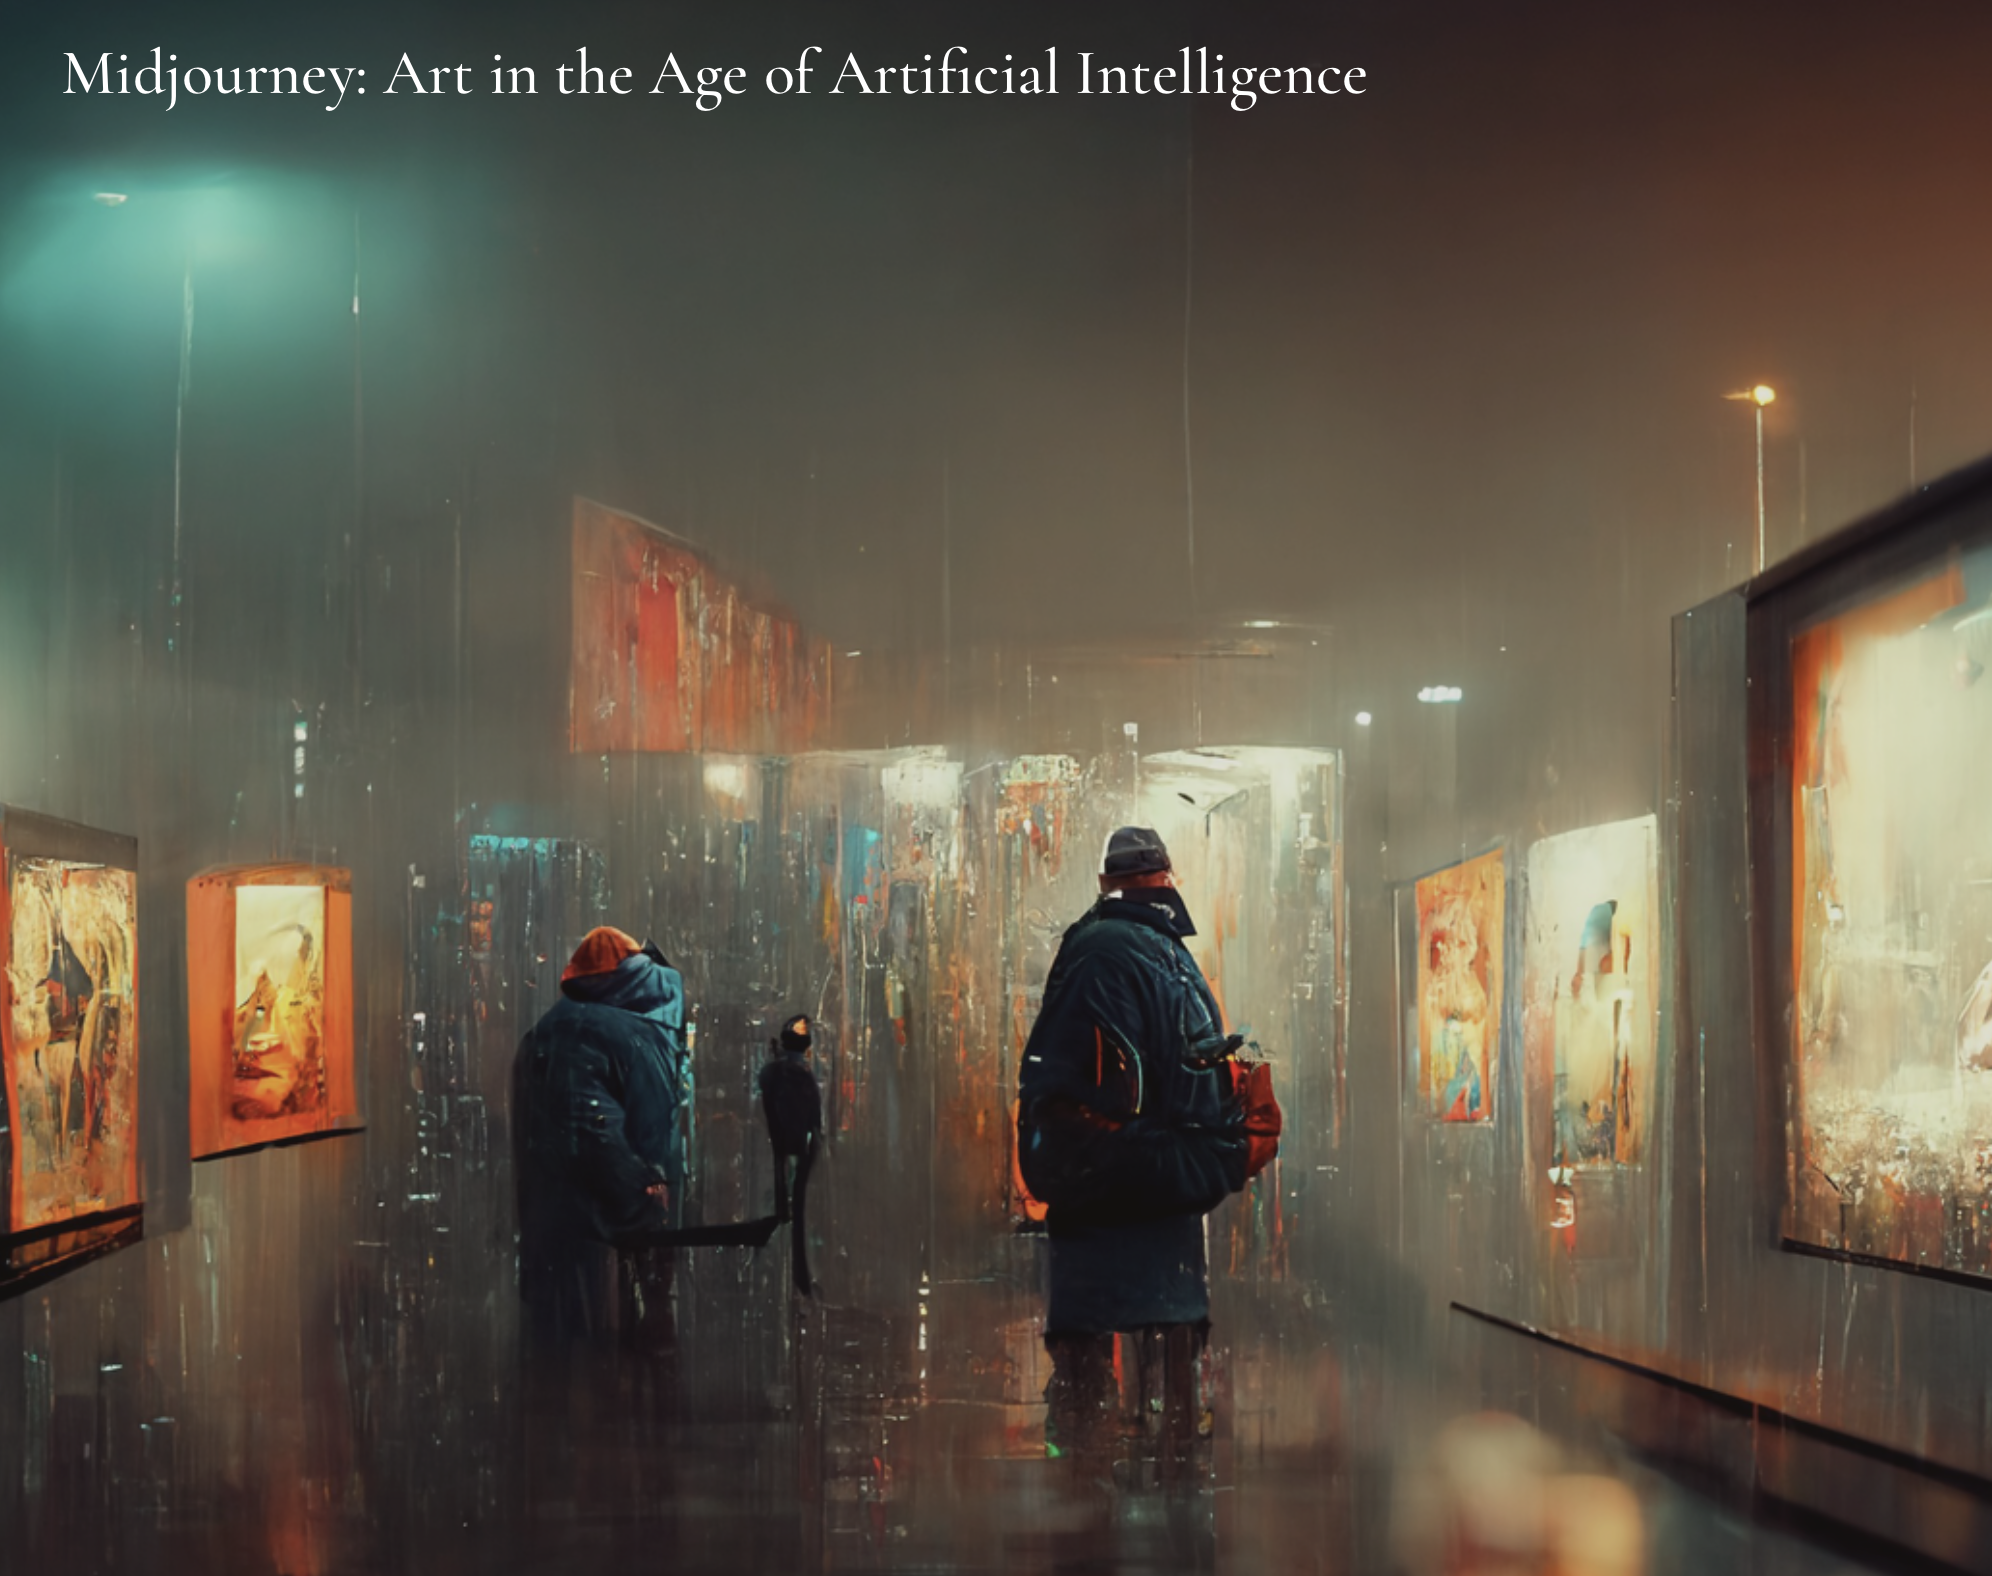
\includegraphics[height=150pt]{figure/midjourney_home.png} 
    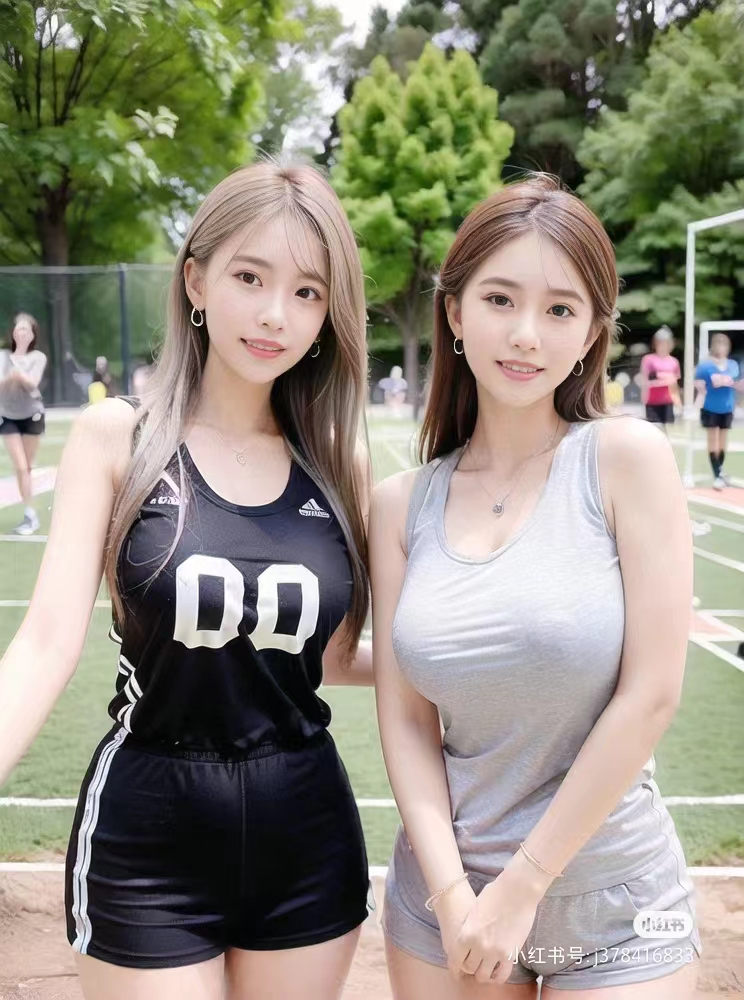
\includegraphics[height=150pt]{figure/ai_pic.jpg} 
  \end{center}  
\end{frame}

\begin{frame}{The Rise of Machine Learning}
  \begin{center}
    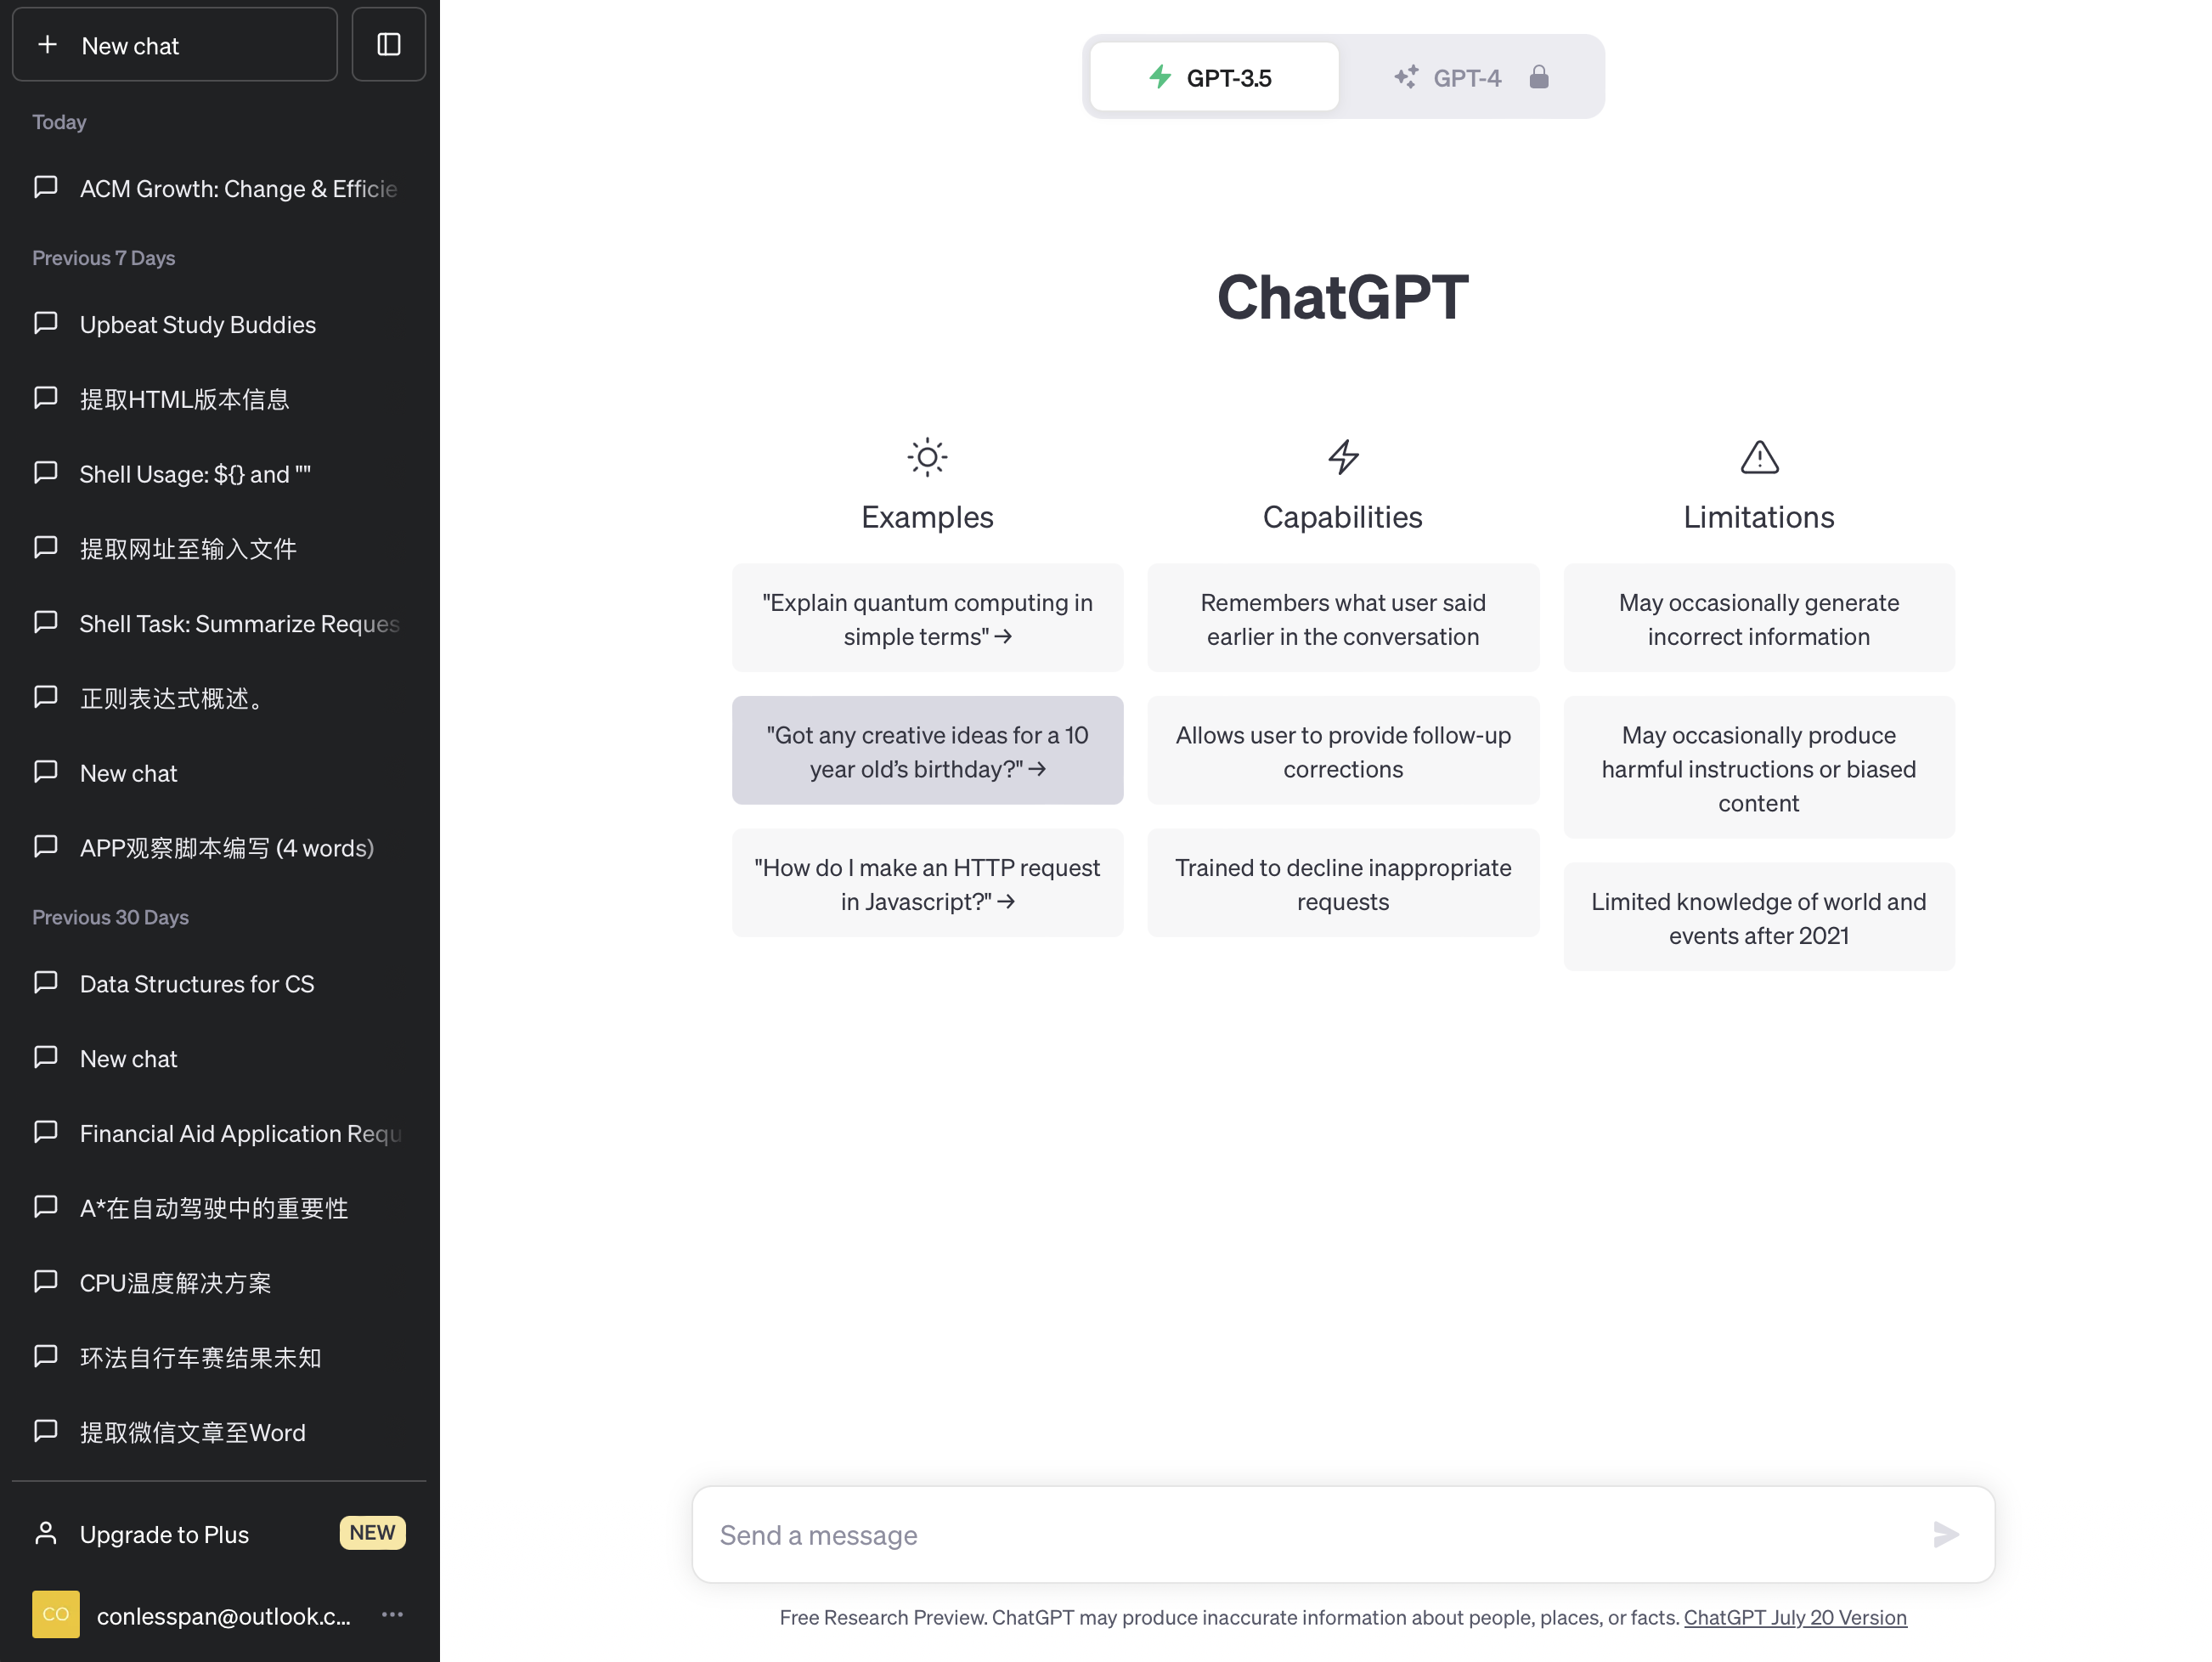
\includegraphics[height=200pt]{figure/chatgpt.png}
  \end{center}
\end{frame}

\begin{frame}{The Rise of Machine Learning}
  \onslide<1->{When we talk about the rise of machine learning, people usually raise these questions:}
  \begin{itemize}
    \item<2-> What is machine learning?
    \item<3-> Do you know its history?
    \item<4-> Why is it so important today?
  \end{itemize}
  \onslide<5->{But I don't want to talk about them, cause I'm not interested about AI.}
\end{frame}

\begin{frame}{Applications of Machine Learning}
  Anyway, AI is a useful tool.
  \begin{itemize}
    \item <2-> Generative AI
    \item <3-> AI for science
    \item <4-> Others
  \end{itemize}
\end{frame}

\section{AI for System}

\begin{frame}{How can AI promote our research of computer system?}
  Let's compare these two games:\footfullcite{smith1998study}
  \begin{center} 
    \onslide<2->{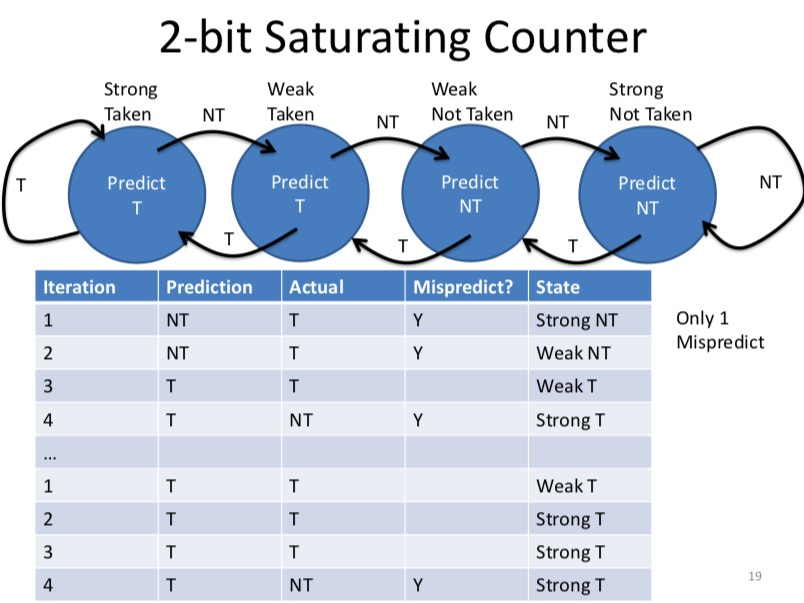
\includegraphics[height=100pt]{figure/2_bit_saturating.jpg}}
    \onslide<3->{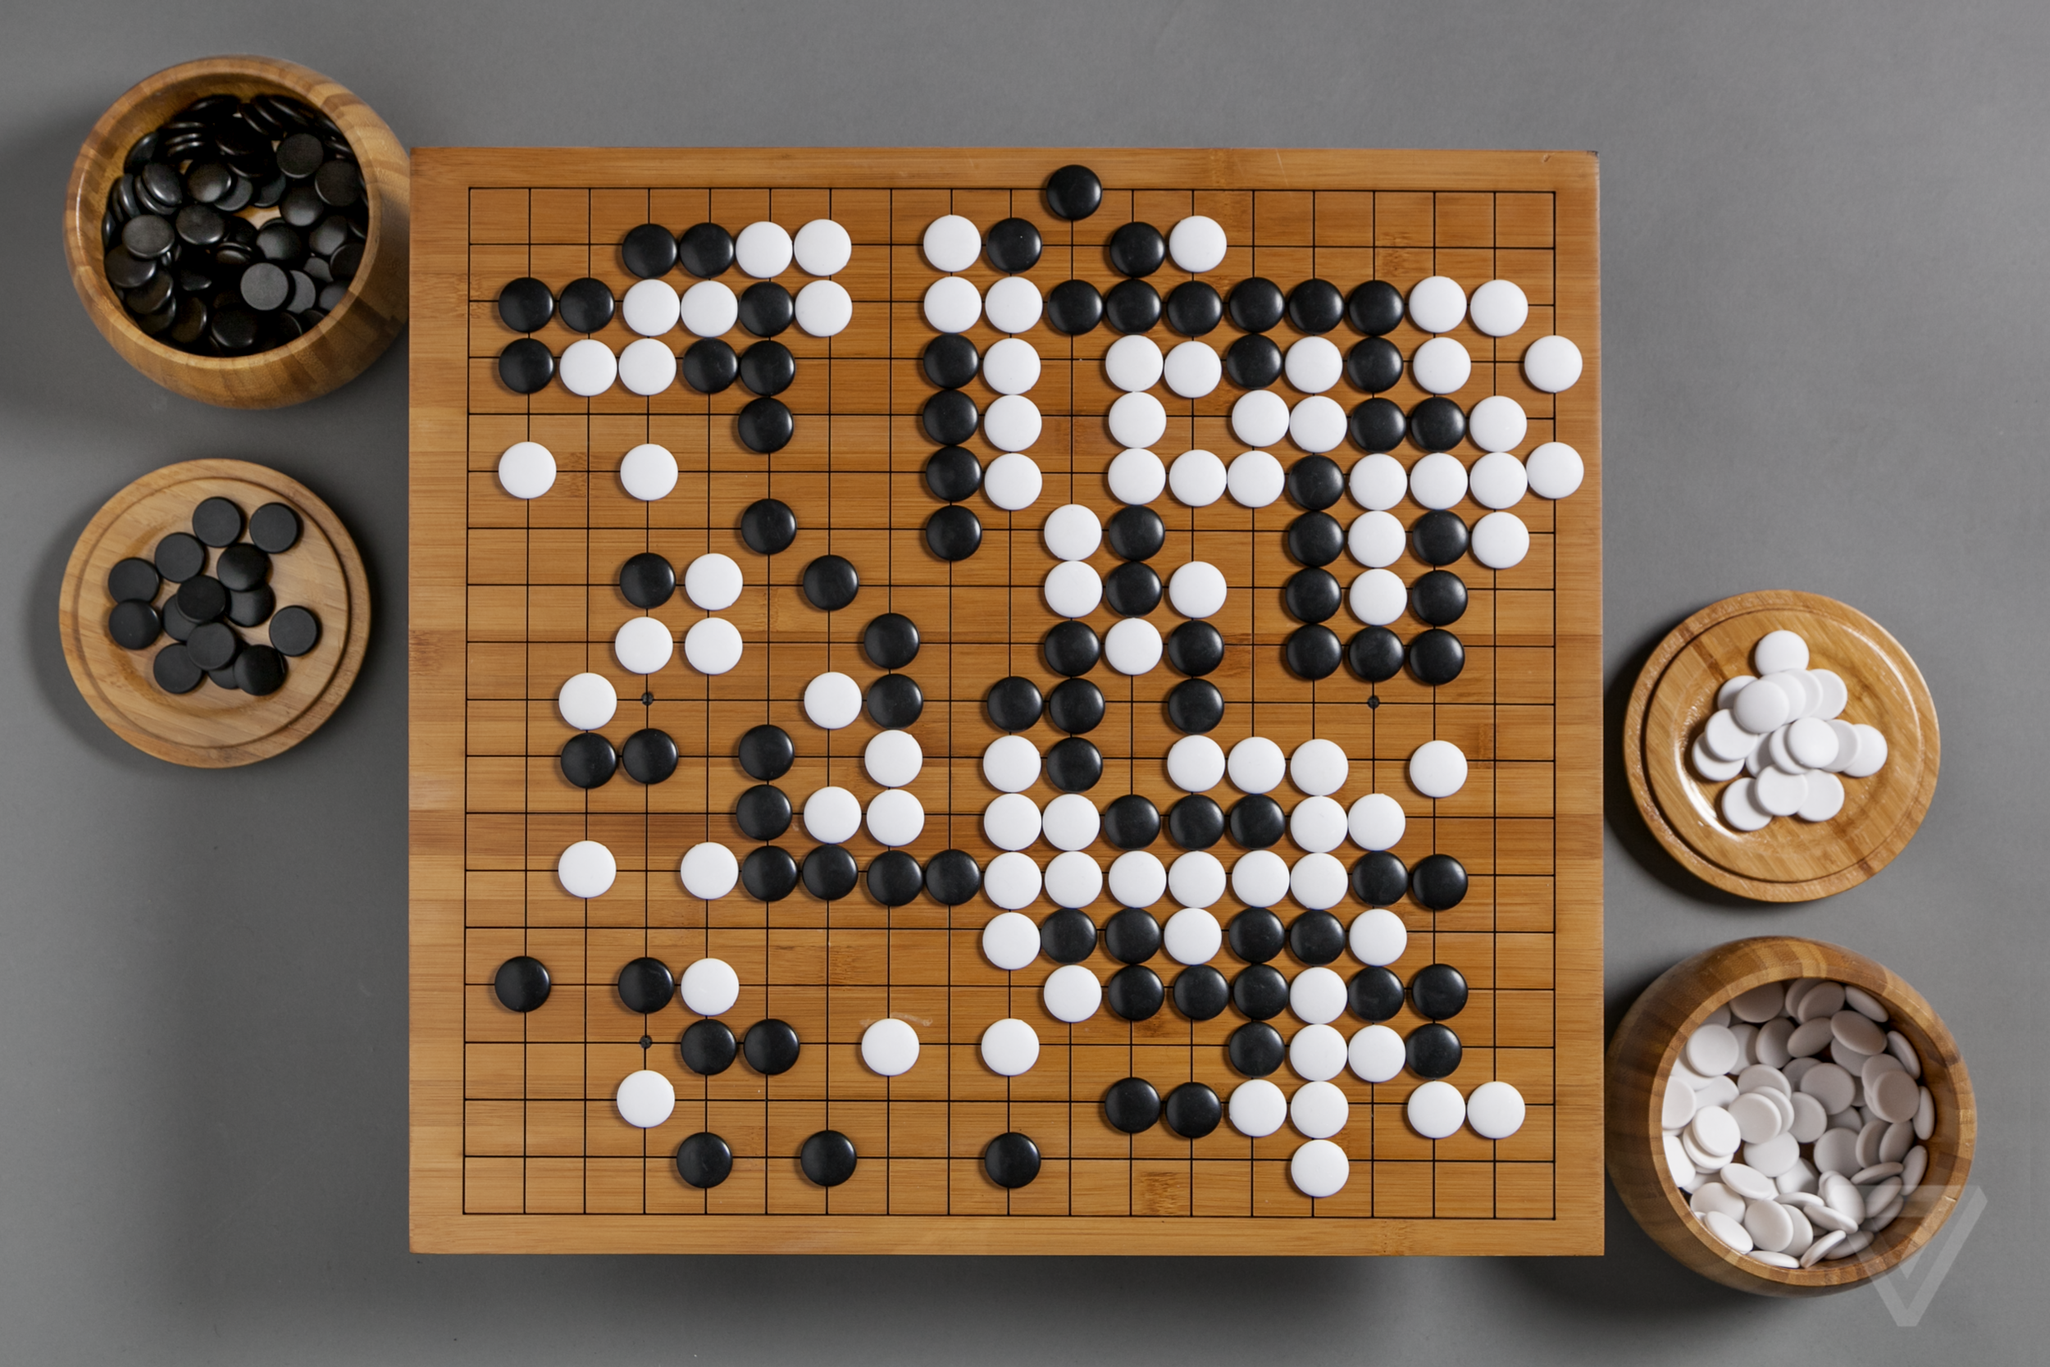
\includegraphics[height=100pt]{figure/go_pic.png}}
  \end{center} 
\end{frame}

\begin{frame}{How can AI promote our research of computer system?}
  And it turns out that...\footfullcite{zouzias2021branch}\footfullcite{silver2017mastering}
  \begin{center} 
    \onslide<2->{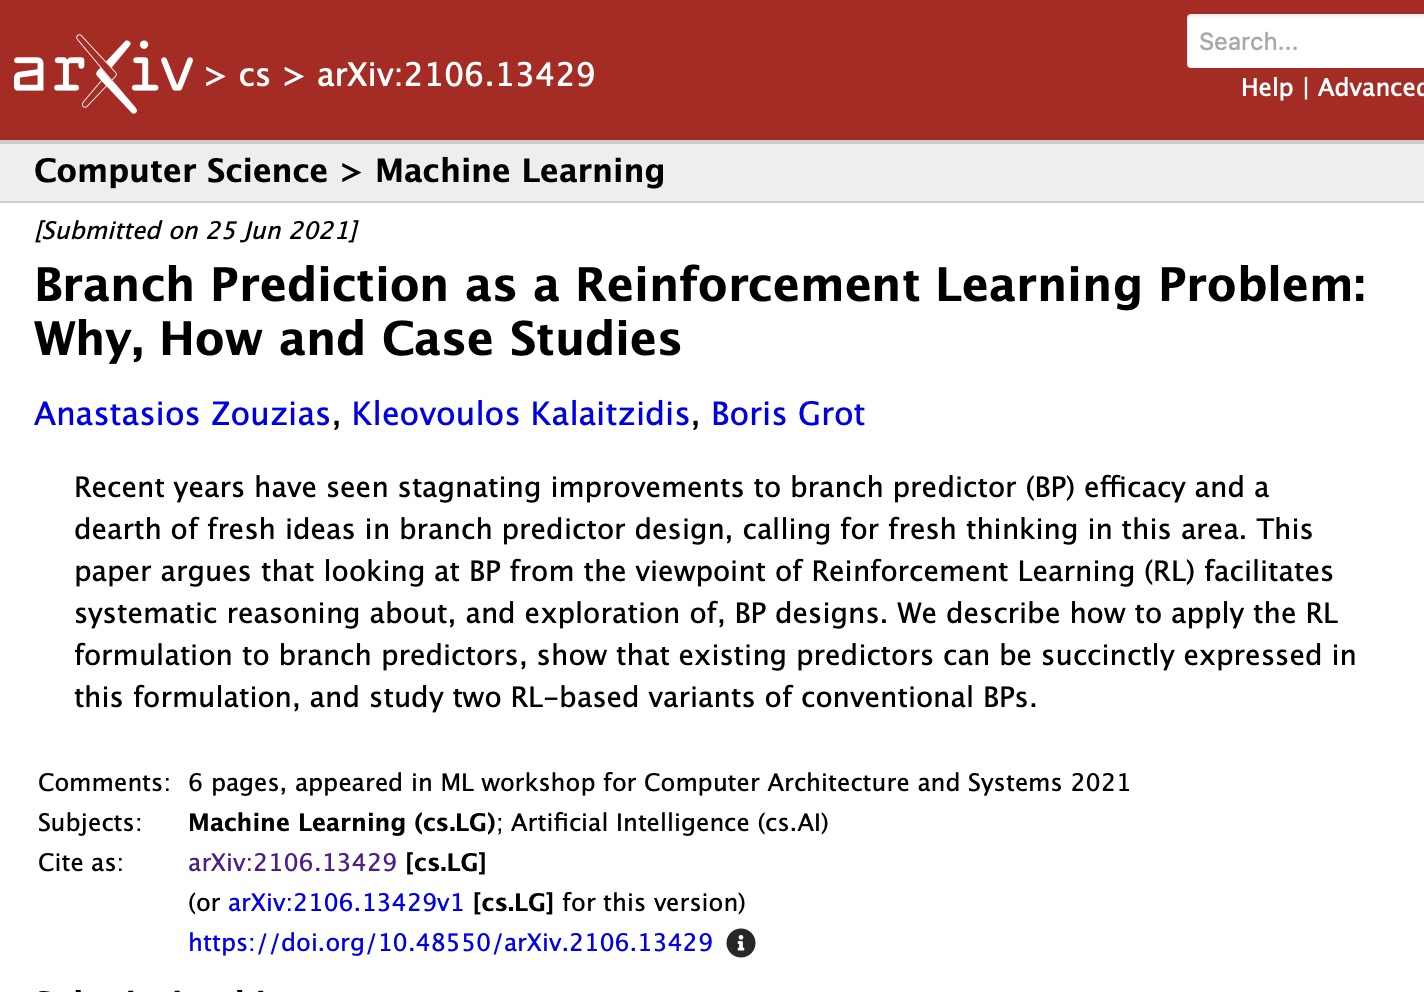
\includegraphics[height=100pt]{figure/reinforcement_prediction.png}}
    \onslide<3->{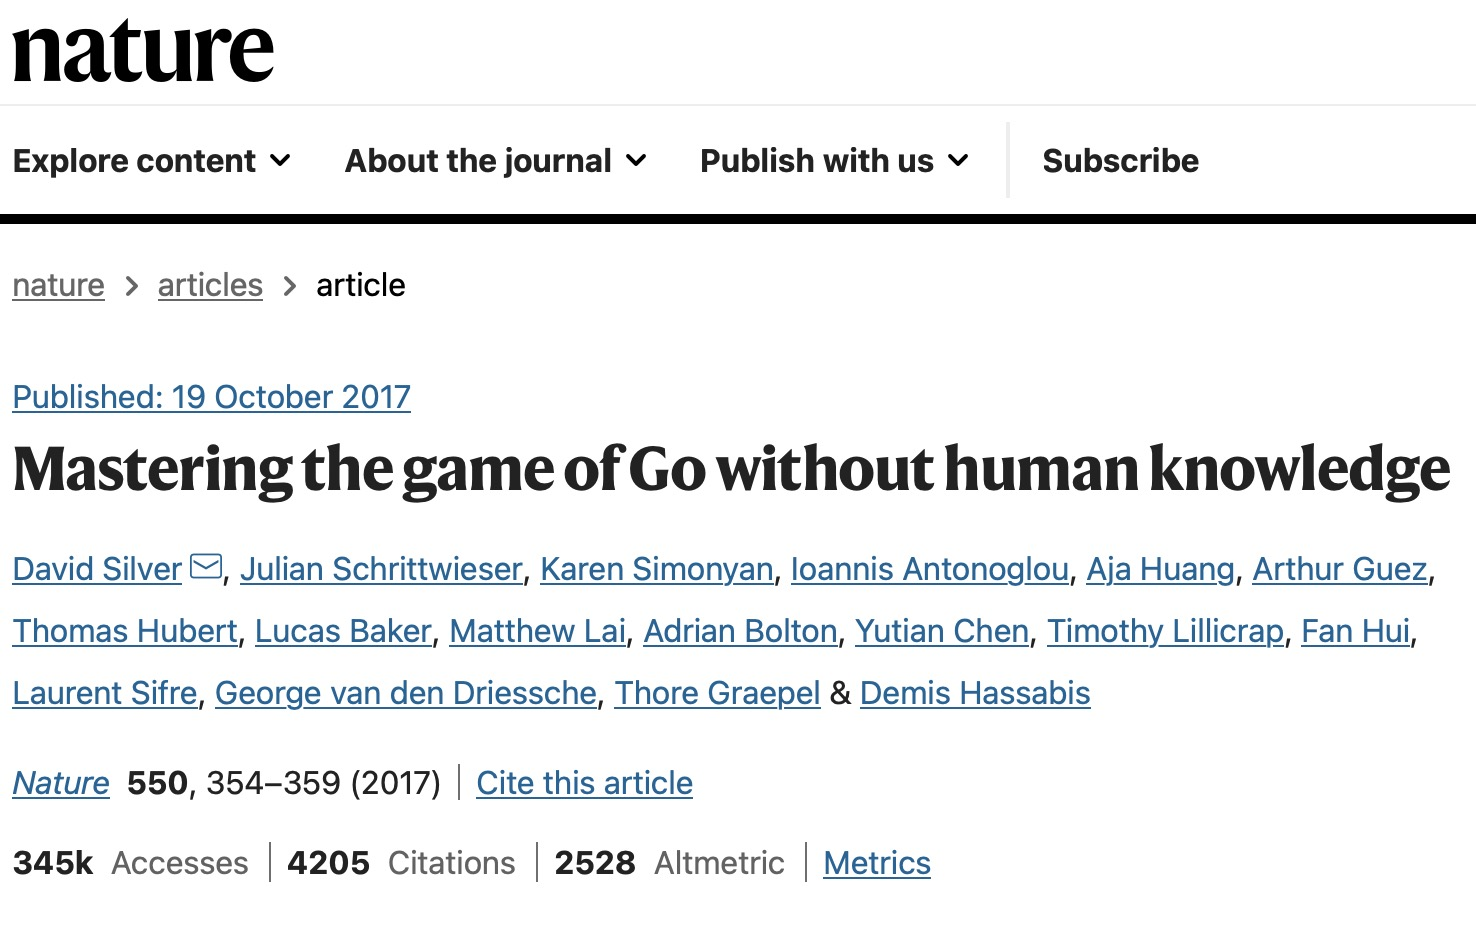
\includegraphics[height=100pt]{figure/master_go.png}}
  \end{center} 
\end{frame}

\begin{frame}{How can AI promote our research of computer system?}
  Their similarities:
  \begin{enumerate}
    \item<2-> Decision-making problems
    \item<3-> A finite state given as input
    \item<4-> A simple decision required as output
  \end{enumerate}

  \onslide<5->{The role that AI plays: looking for a fitting function $y=f(x)$, which calculates the correct/best $y$ with given $x$.}
\end{frame}

\begin{frame}{How does AI perform its job?}
  The perceptron was introduced at first:\footfullcite{jimenez2001dynamic}
  \begin{center} 
    \onslide<2->{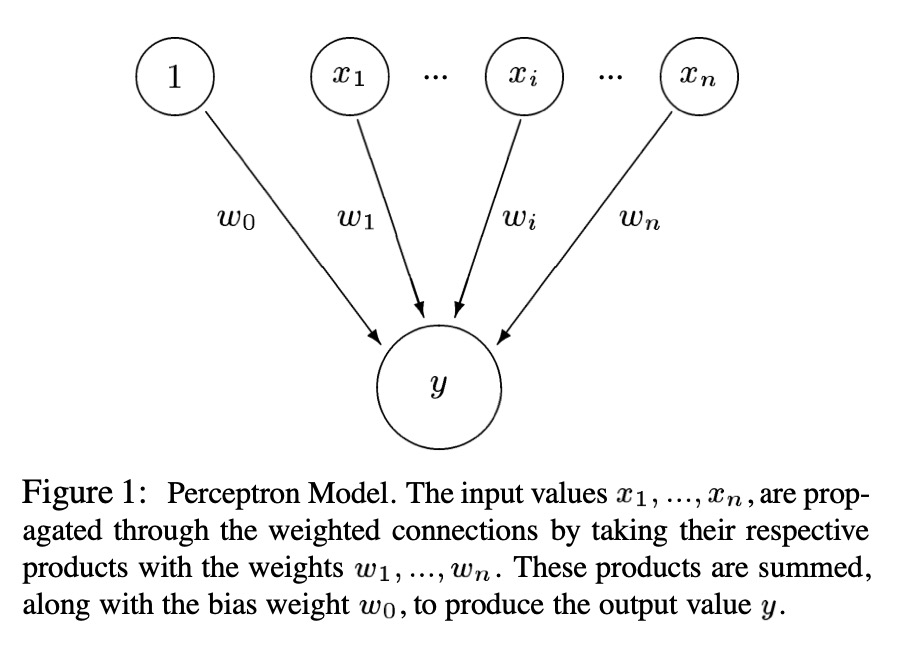
\includegraphics[height=120pt]{figure/perceptron.jpg}}
    \onslide<3->{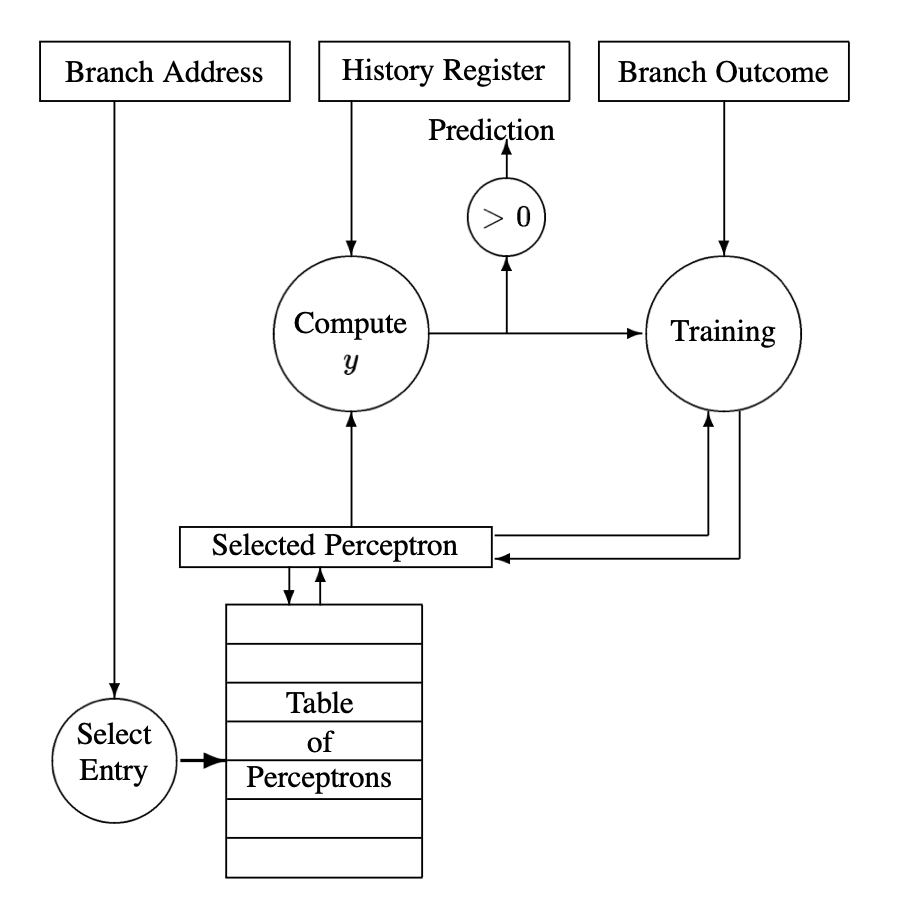
\includegraphics[height=120pt]{figure/bp_structure.png}}
  \end{center}
\end{frame}

\begin{frame}{Applications}
  AMD Zen microarchitecture, the start of "AMD YES".
  \begin{center}
    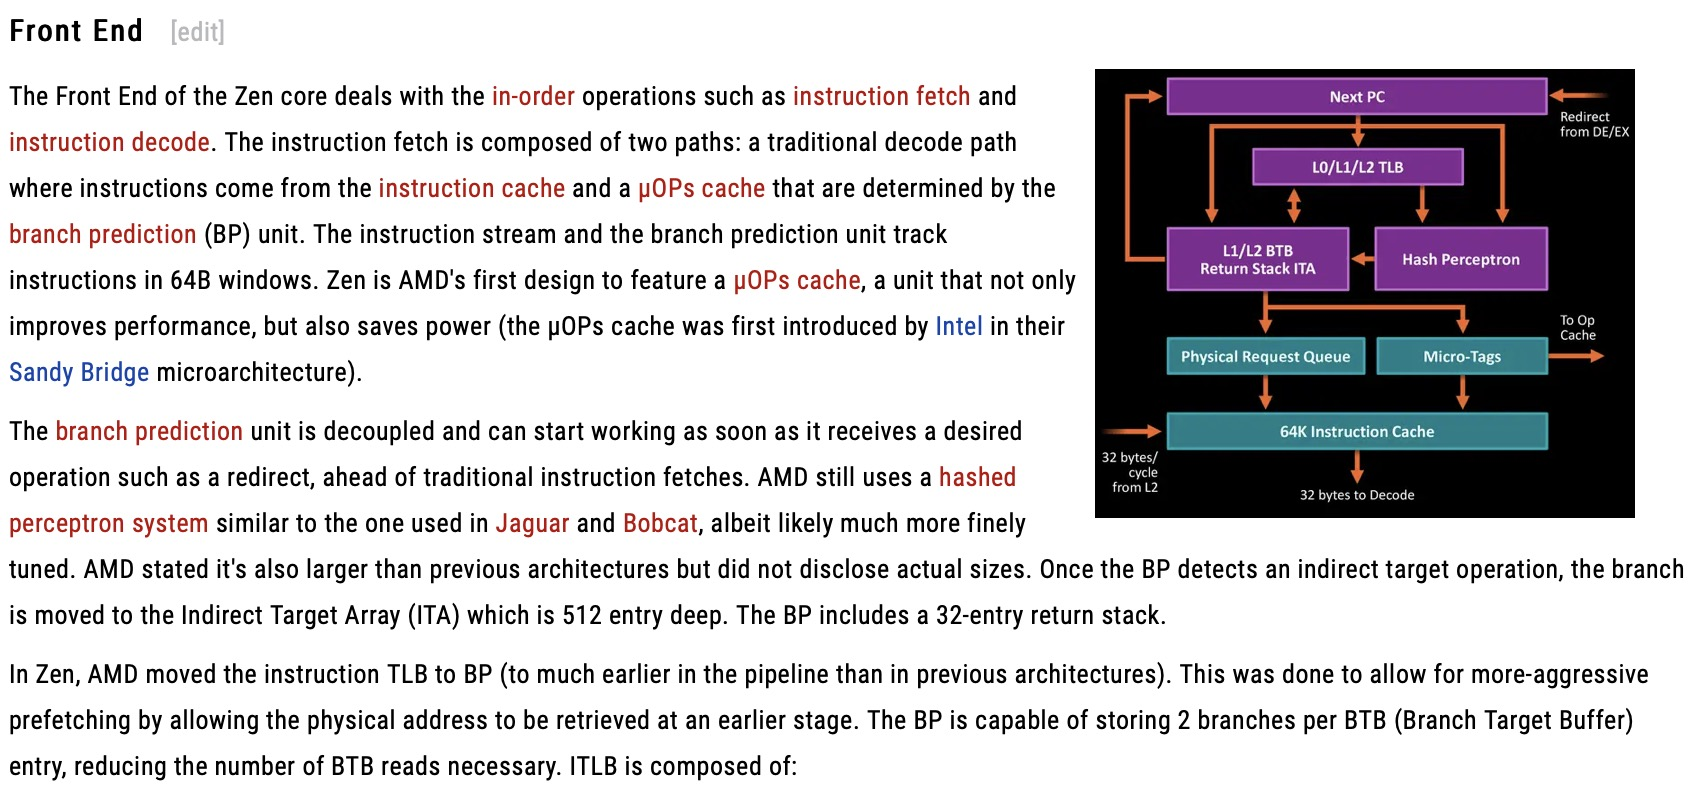
\includegraphics[height=150pt]{figure/amd_zen_bp.jpg}
  \end{center}
\end{frame}

\begin{frame}{Advanced version}
  Advanced neural network is also being introduced to many subfields of computer system\dots
\end{frame}

\begin{frame}{Reinforcement is all you need}
  Let's go over the basic concept of reinforcement learning.
  \begin{itemize}
    \item <2-> A virtual agent who makes decisions
    \item <3-> A state space $S=\{s_i\}$
    \item <4-> An action space $A=\{a_i\}$
    \item <5-> Rewards $r_{a_i|s_i}$
  \end{itemize}
  \onslide<6-> {
    When agent receives a reward or a feedback, it updates the estimation \begin{align*}
      \mathbb{E} (r_{a_i|s_i})
    \end{align*}
    or under some situation the probability \begin{align*}
      \mathbb{P} (r_{a_i|s_i}>0)
    \end{align*}
  }
\end{frame}

\begin{frame}{Applications}
  The problems that reinforcement learning can deal with:
  \begin{itemize}
    \item Heuristic
    \item Empirical
  \end{itemize}
\end{frame}

\begin{frame}{Database Management System}
  The configuration of the knobs\footfullcite{van2017automatic}
  \begin{center}
    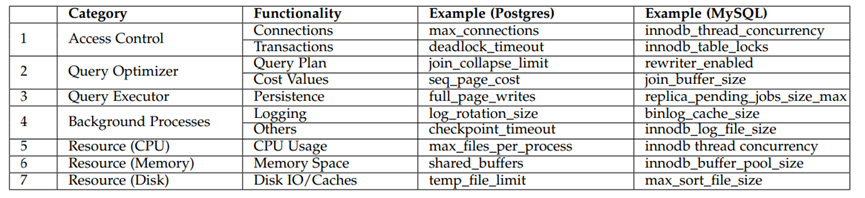
\includegraphics[height=75pt]{figure/dbms_knobs.png}
  \end{center}
  \begin{center}
    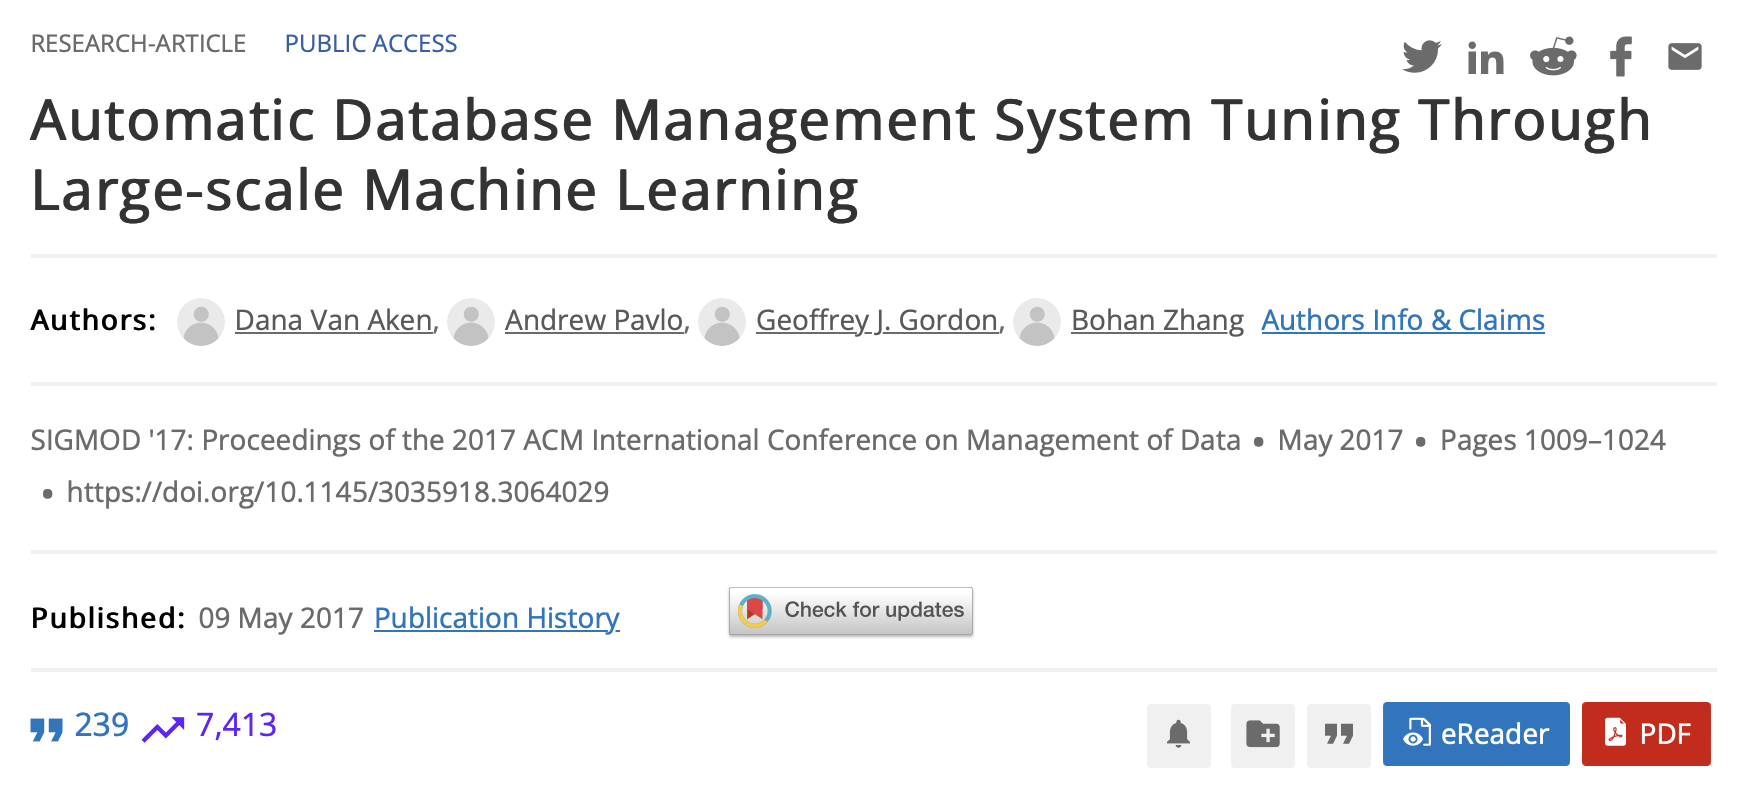
\includegraphics[height=120pt]{figure/auto_dbms.png}
  \end{center}
\end{frame}

\begin{frame}{Operating System}
  The management of page table index\footfullcite{margaritov2018virtual}
  \begin{center}
    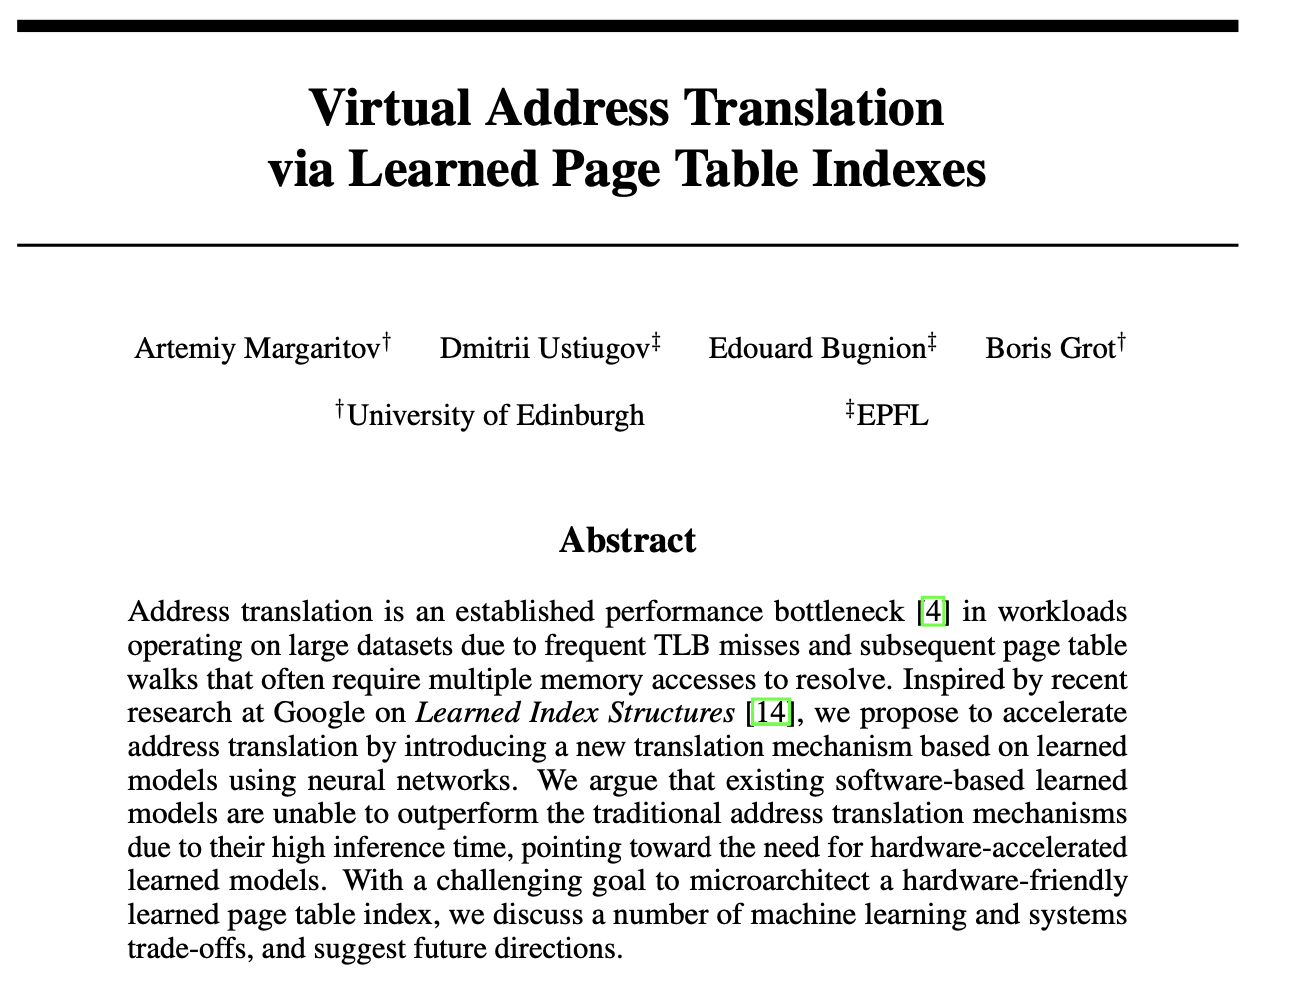
\includegraphics[height=150pt]{figure/page_index.png}
  \end{center}
\end{frame}

\begin{frame}{Applications}
  Anywhere we use heuristic to make a decision can be replaced by ml!\footfullcite{dean2017machine}
  \begin{itemize}
    \item <2-> Compilers: instruction scheduling, register allocation, loop nest parallelization strategies, ...
    \item <2-> Networking: TCP window size decisions, backoff for retransmits, data compression, ...
    \item <2-> Operating systems: process scheduling, buffer cache insertion/replacement, file system prefetching, ...
    \item <2-> Job scheduling systems: which tasks/VMs to co-locate on same machine, which tasks to pre-empt, ...
    \item <2-> ASIC design: physical circuit layout, test case selection, ...
  \end{itemize}
\end{frame}

\begin{frame}{Framework for RL in Sys}
  There are some frameworks for these systems\footfullcite{mao2019park}:
  \begin{center}
    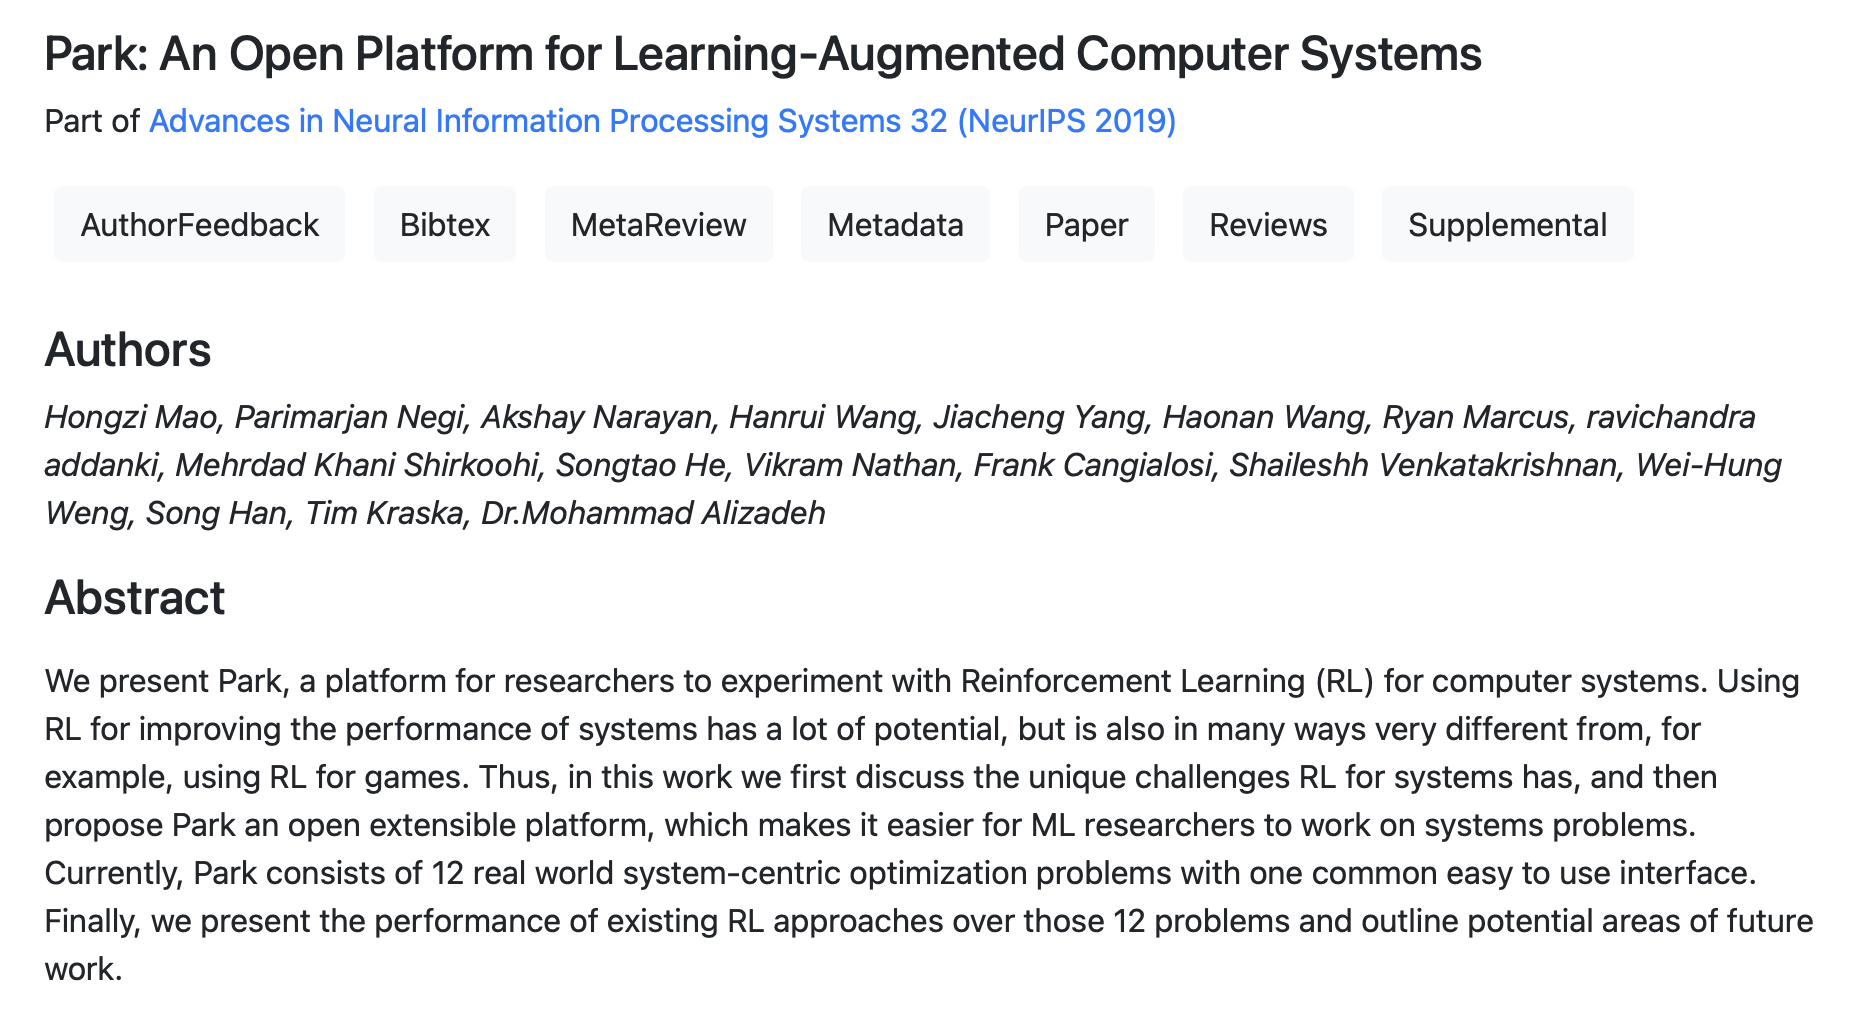
\includegraphics[height=180pt]{figure/park_project.png}
  \end{center}
\end{frame}

\section{System for AI}

\begin{frame}{How can our works on system promote research of AI?}
  Large models are conquering ml\dots
  \begin{center}
    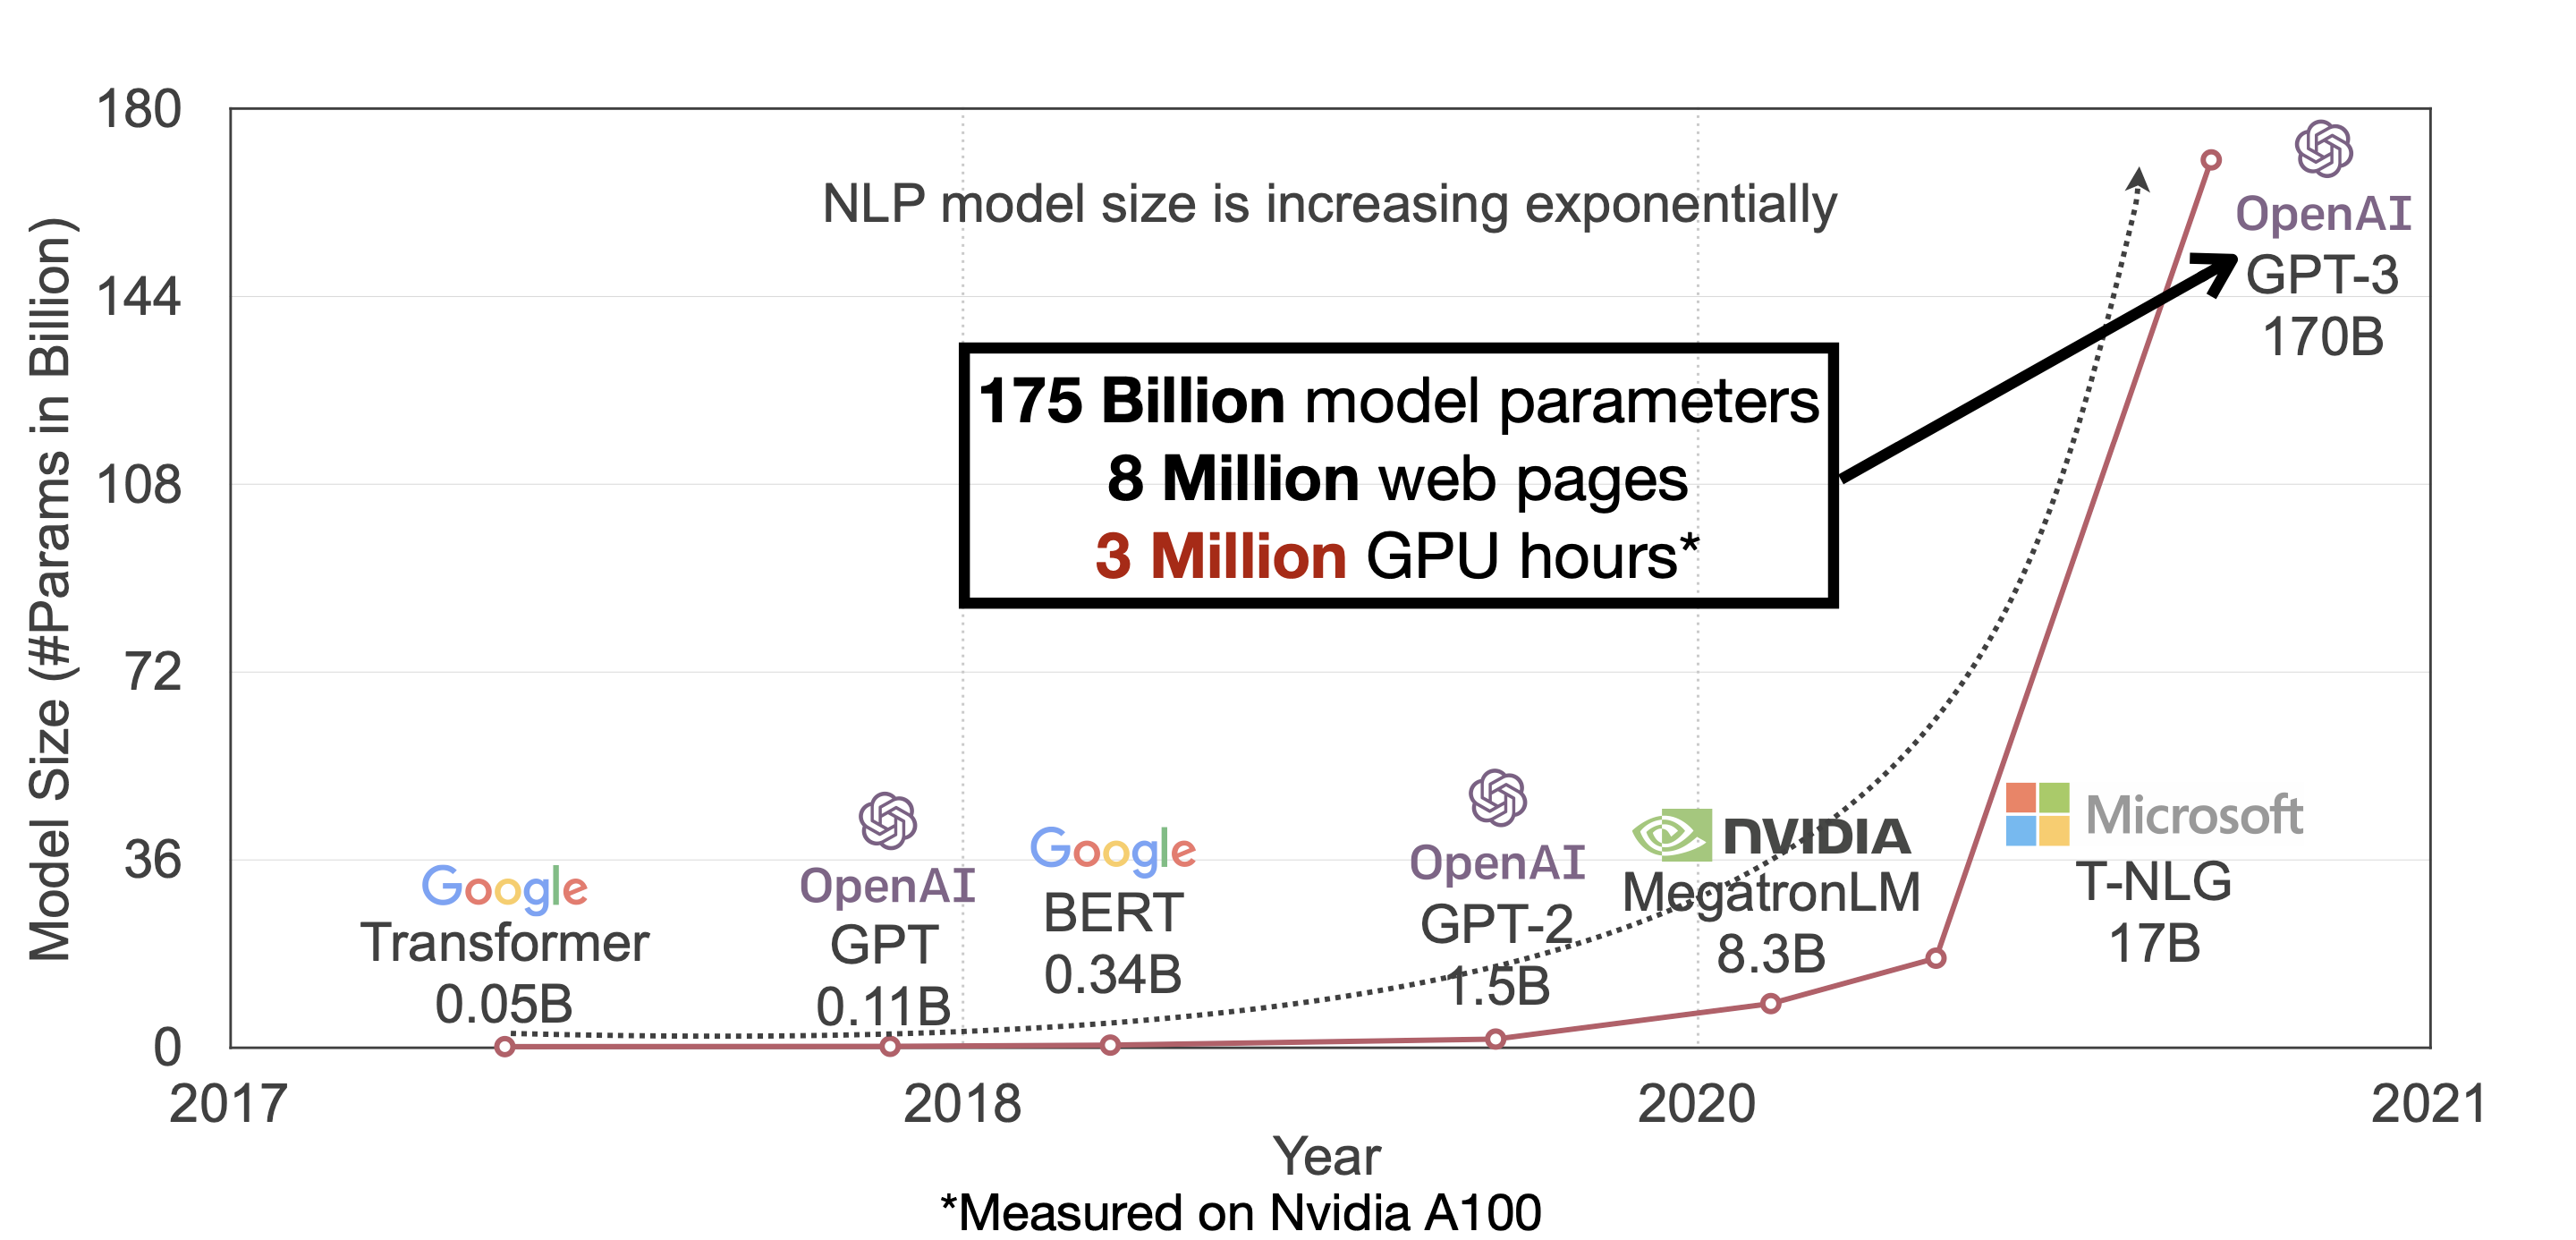
\includegraphics[height=90pt]{figure/nlp_large_models.png}
    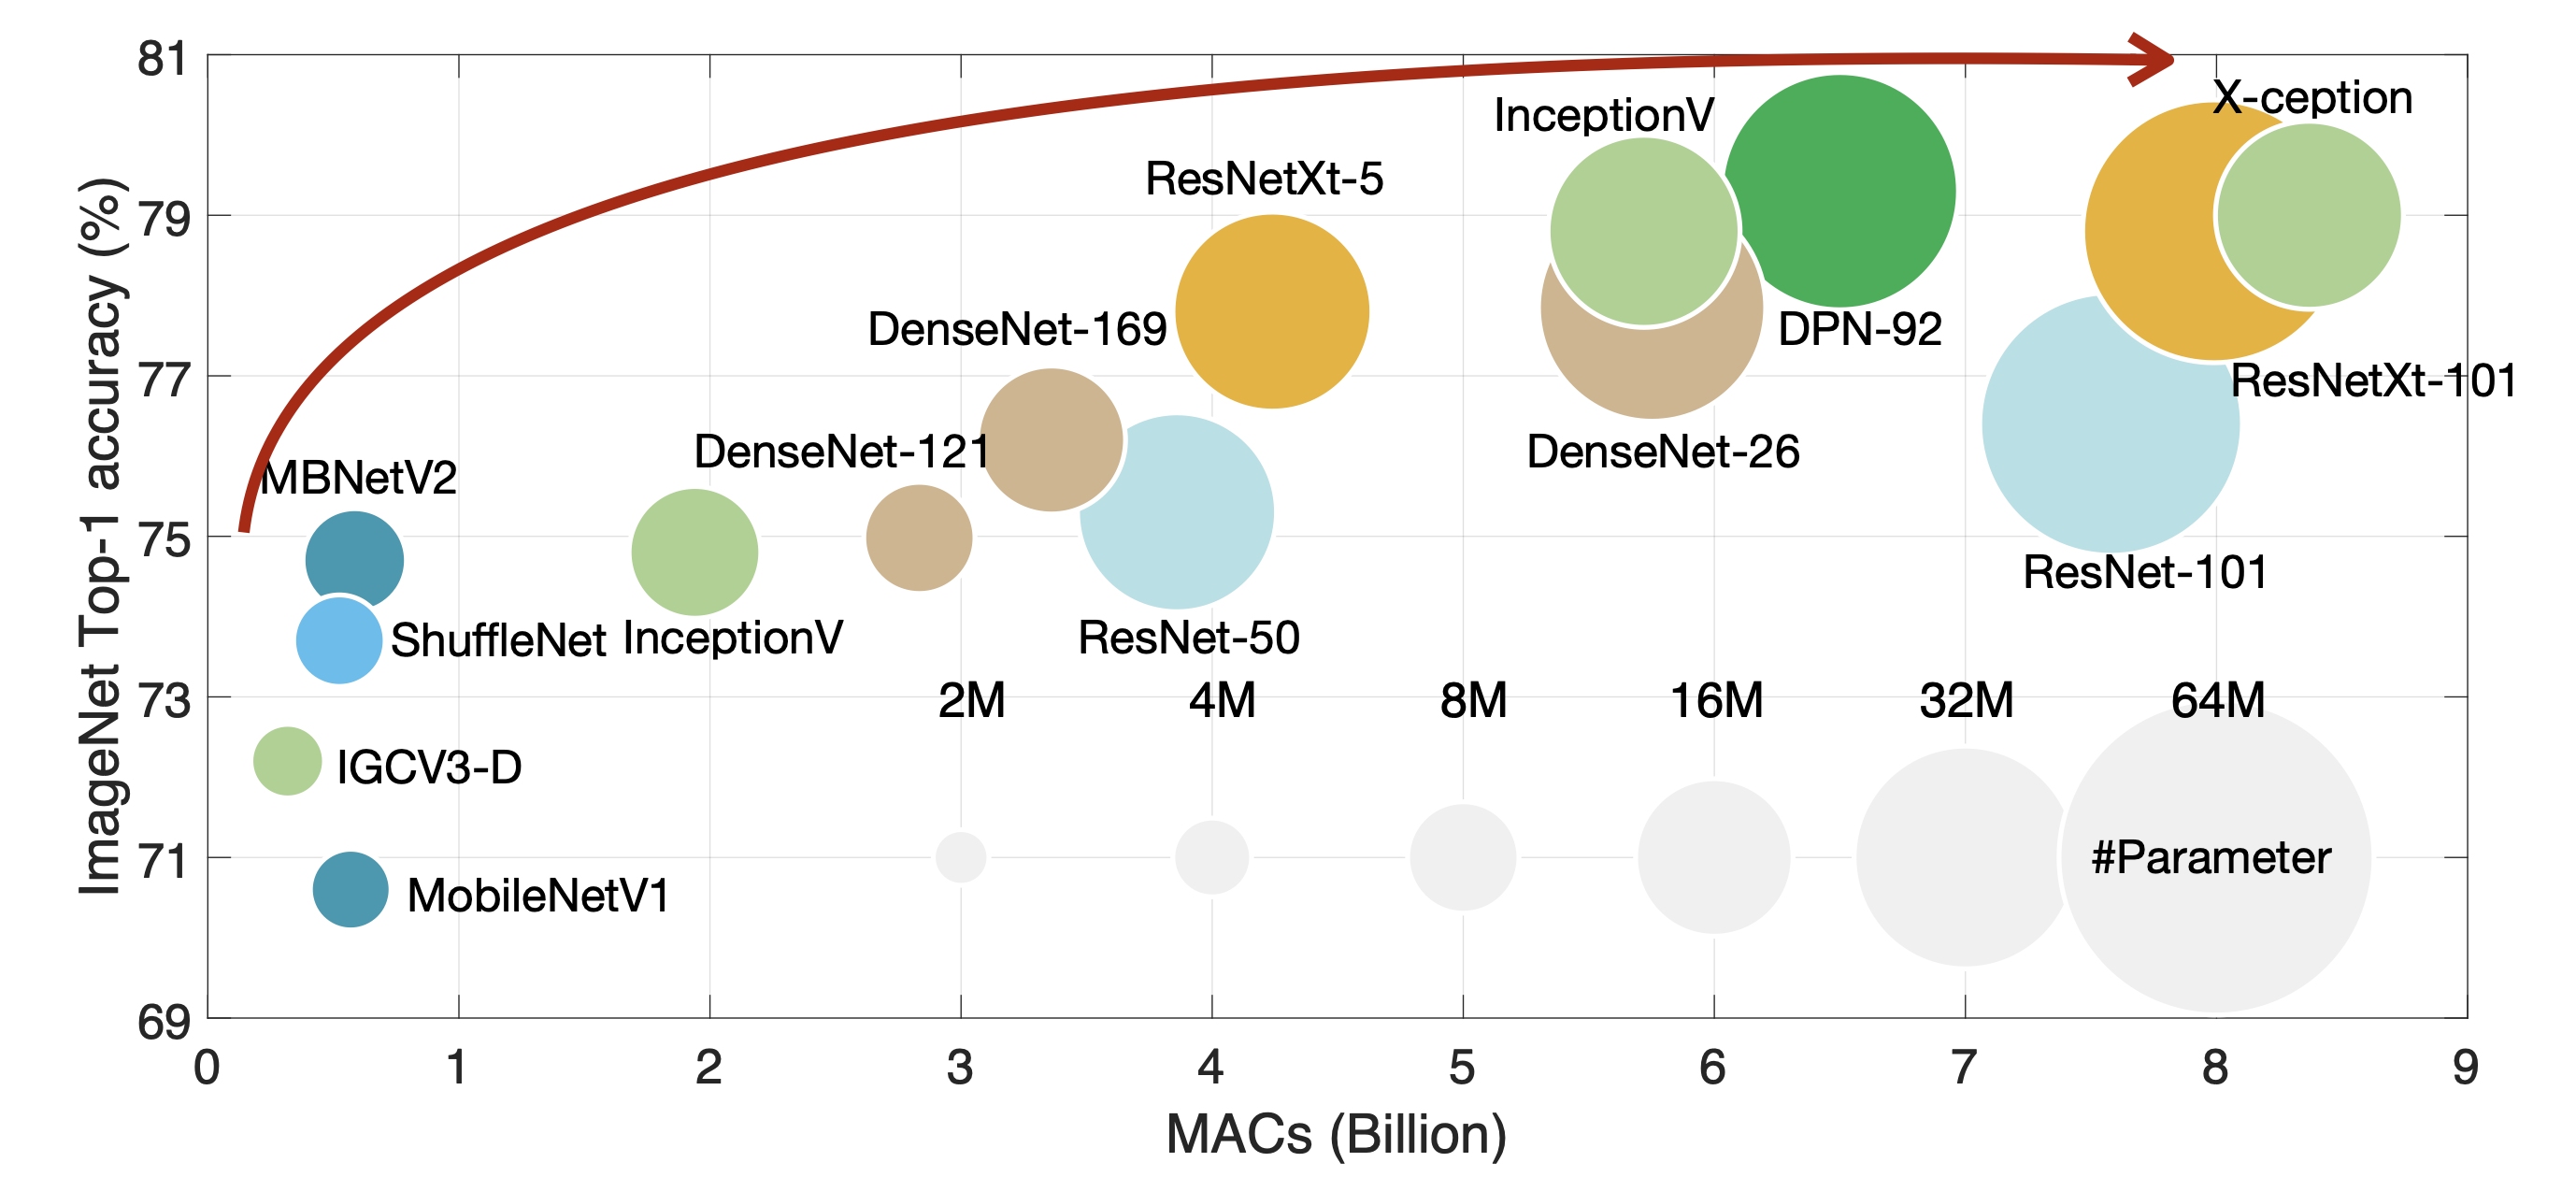
\includegraphics[height=90pt]{figure/cv_large_models.png}
  \end{center}
\end{frame}

\begin{frame}{Problems in system}
  With the growth of size, problems occurred.
  \begin{itemize}
    \item <2-> Low speed
    \item <3-> Limited memory
    \item <4-> Popularization
  \end{itemize}
\end{frame}

\begin{frame}{Improvements}
  Speed can be achieved with loss of precision and generality
  
  \begin{columns}
    \column{0.5\textwidth}
    \centering Reduced precision
    \column{0.5\textwidth}
    \centering 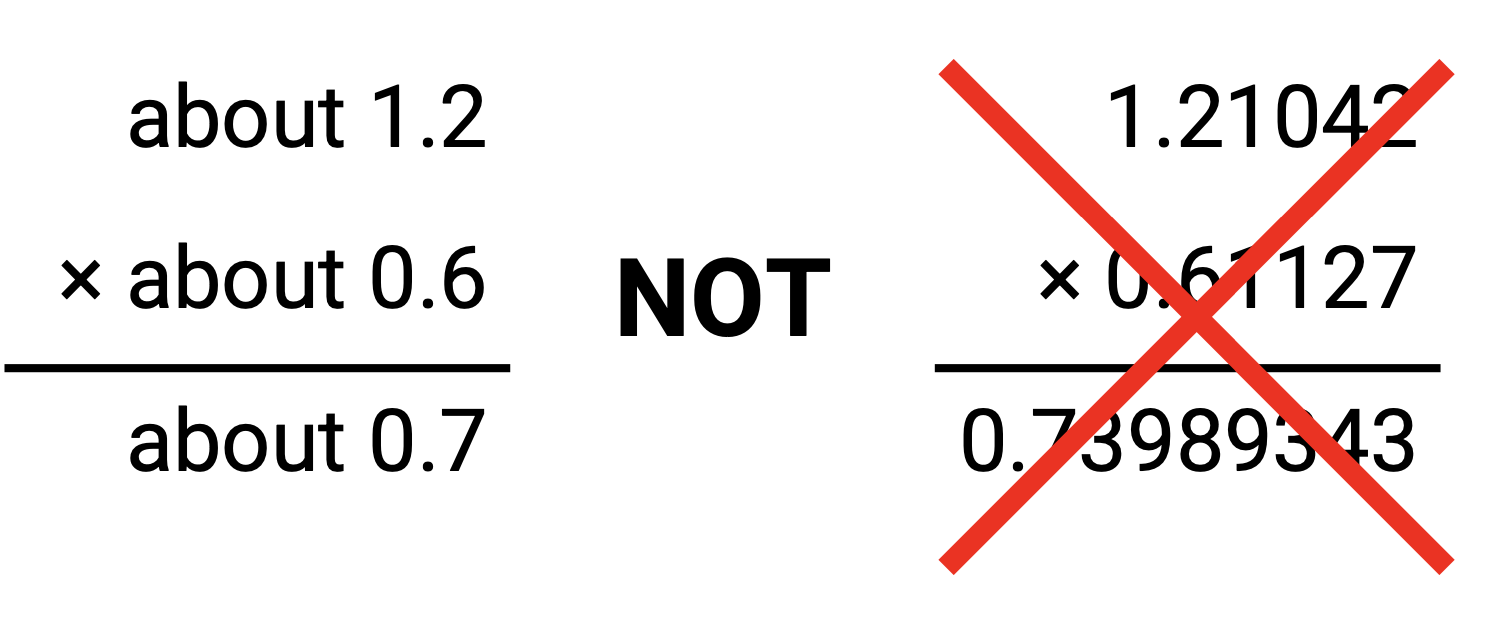
\includegraphics[height=4\baselineskip]{figure/reduced_prediction.png}
  \end{columns}

  \begin{columns}
    \column{0.5\textwidth}
    \centering Specific operations
    \column{0.5\textwidth}
    \centering 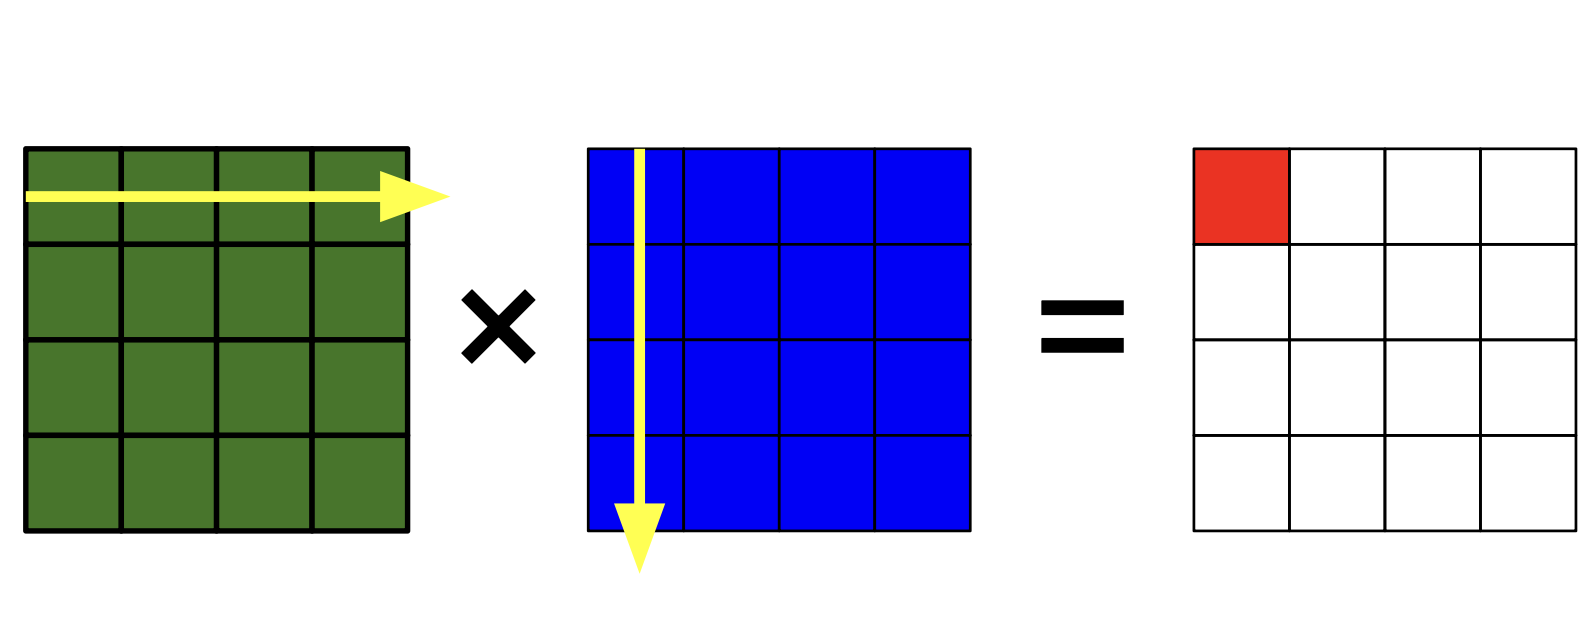
\includegraphics[height=4\baselineskip]{figure/conv_oper.png}
  \end{columns}
\end{frame}

\begin{frame}{Improvements}
  Thus we have Nvidia GPUs with CUDA units and tensor cores, Google TPU and Apple NPU.
  \begin{center}
    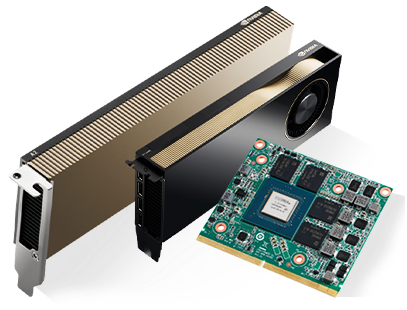
\includegraphics[height=4\baselineskip]{figure/nvidia_gpu.png}
    \hfill
    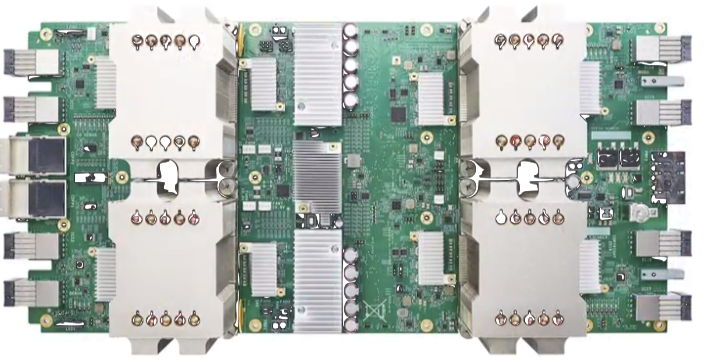
\includegraphics[height=4\baselineskip]{figure/google_tpu.png}
    \hfill
    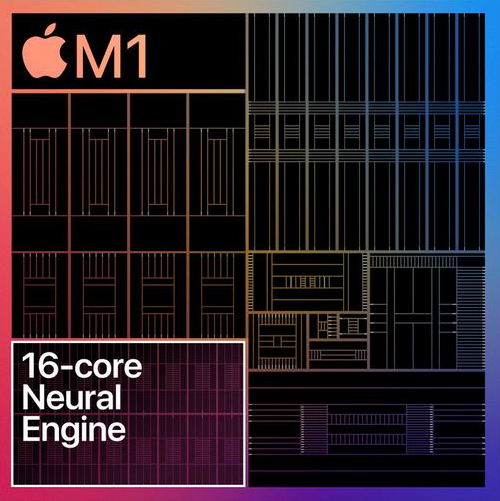
\includegraphics[height=4\baselineskip]{figure/apple_m1_npu.png}
  \end{center}
\end{frame}

\begin{frame}{Improvements}
  In traditional data storage and computing, we distribute data/tasks to multiple machines for larger storage size and better speed.
  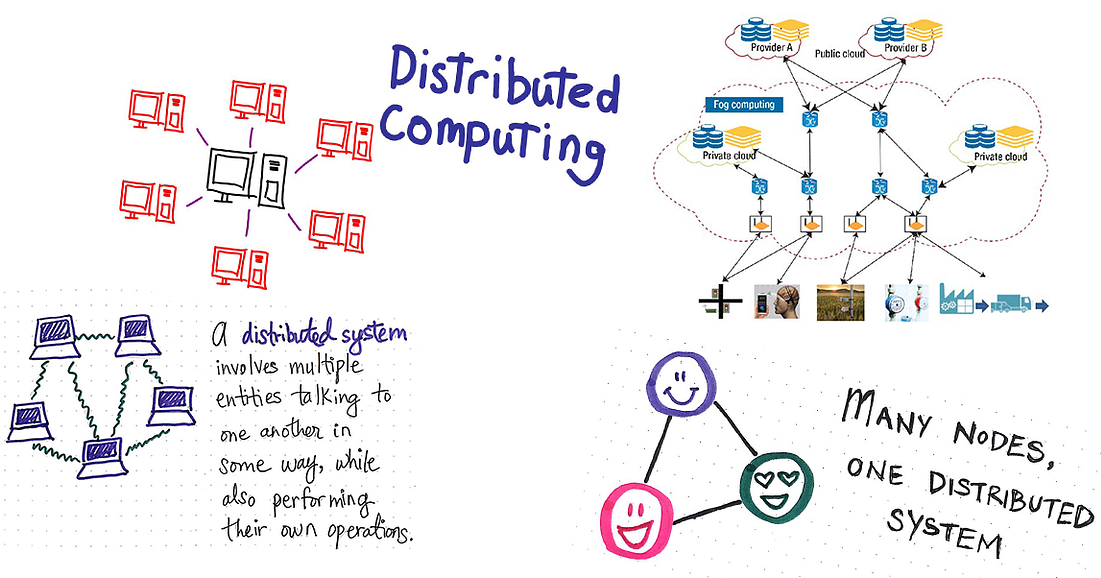
\includegraphics[height=150pt]{figure/distributed_system.png}
\end{frame}

\begin{frame}{Improvements}
  The same idea can also be applied into ml
  \begin{itemize}
    \item <2-> Distributed machine learning system (parallel compute / parallel data)
    \item <3-> Computing device placement
    \item <4-> Other topics in traditional distributed sys (communication, consistency)
  \end{itemize}
\end{frame}

\begin{frame}{Convenience}
  Programmers don't want to build their projects from every detail. 
  
  \begin{center}
    
\includegraphics[height=45pt]{figure/cpp_stl.png}
    \hfill
    
\includegraphics[height=45pt]{figure/qt_logo.png}
    \hfill
    
\includegraphics[height=45pt]{figure/directx.jpeg}
  \end{center}
  
  When writing cpp programs, it's convenient for us to use those frameworks and libraries.
  
  AI programmers also need them.
\end{frame}

\begin{frame}{Frameworks}
  \begin{minipage}[b]{0.6\textwidth}
    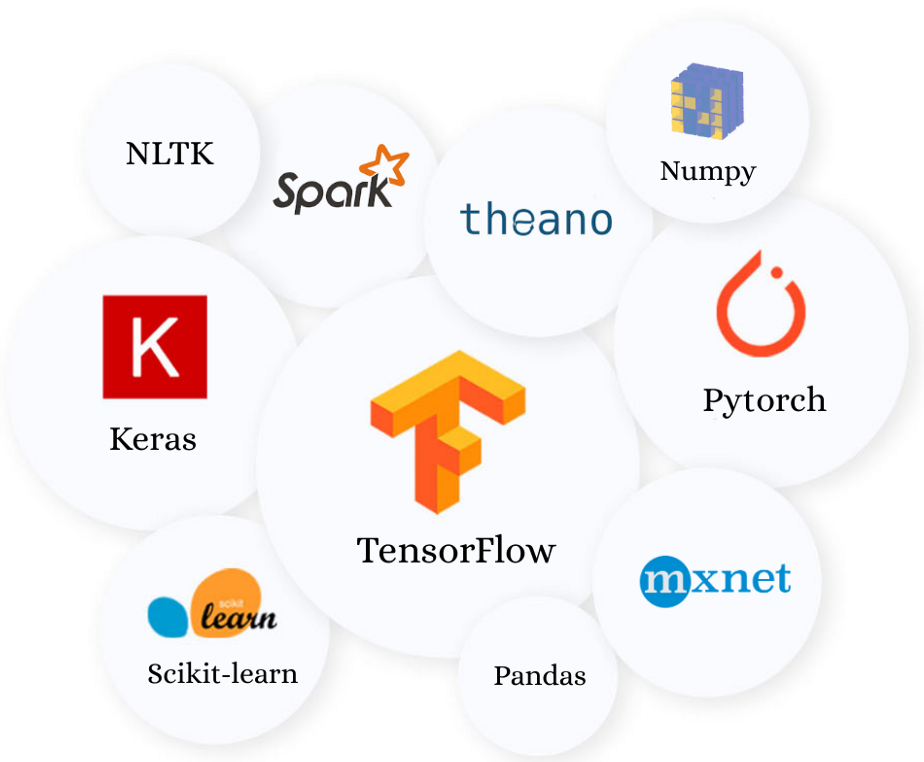
\includegraphics[height=150pt]{figure/dl_framework.png}
  \end{minipage}
  \begin{minipage}[b]{0.3\textwidth}
    
\includegraphics[height=80pt]{figure/nvidia_cuda.png}
    
\includegraphics[height=20pt]{figure/tvm_logo_small.png}
  \end{minipage}
\end{frame}

\begin{frame}{Frameworks}
  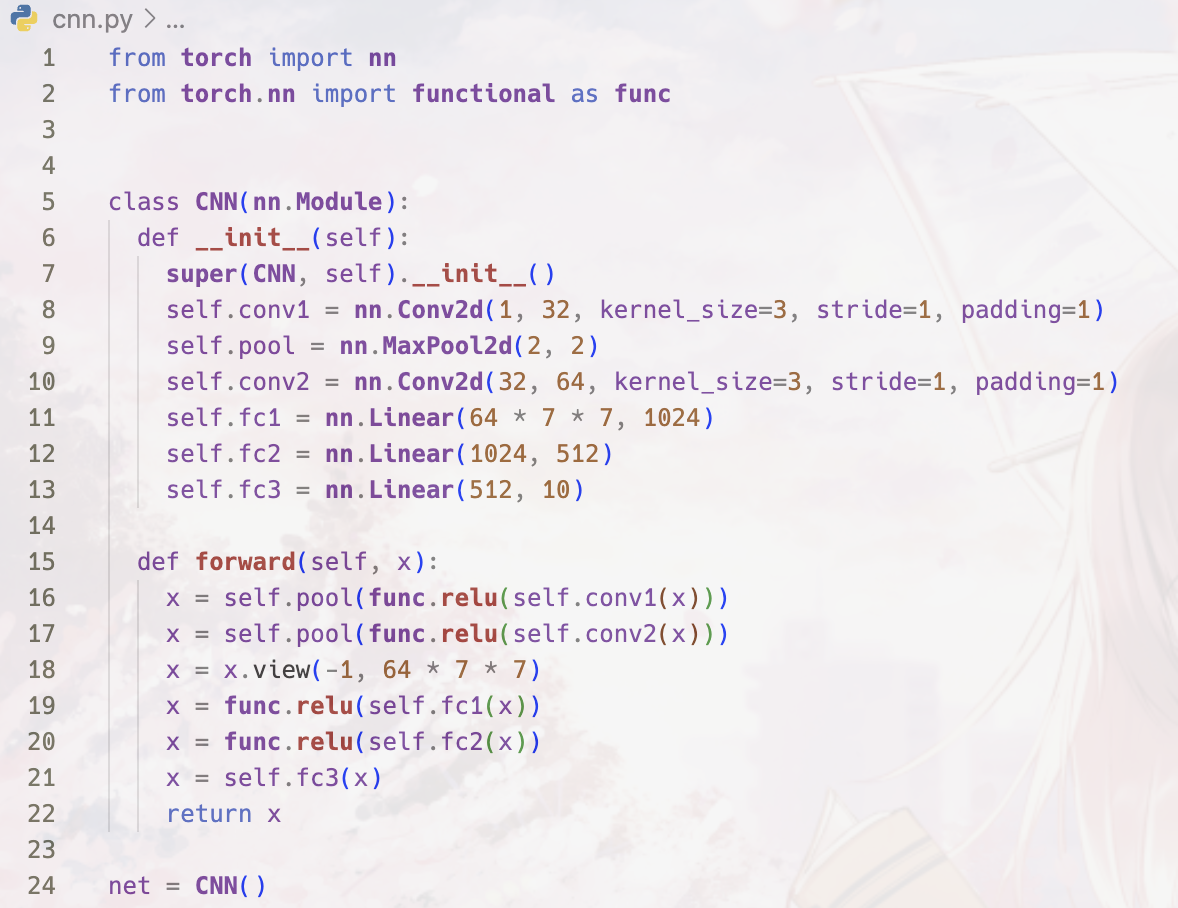
\includegraphics[height=200pt]{figure/cnn_pytorch.png}
\end{frame}

\section{Prospects}

\begin{frame}{Higher level ideas}
  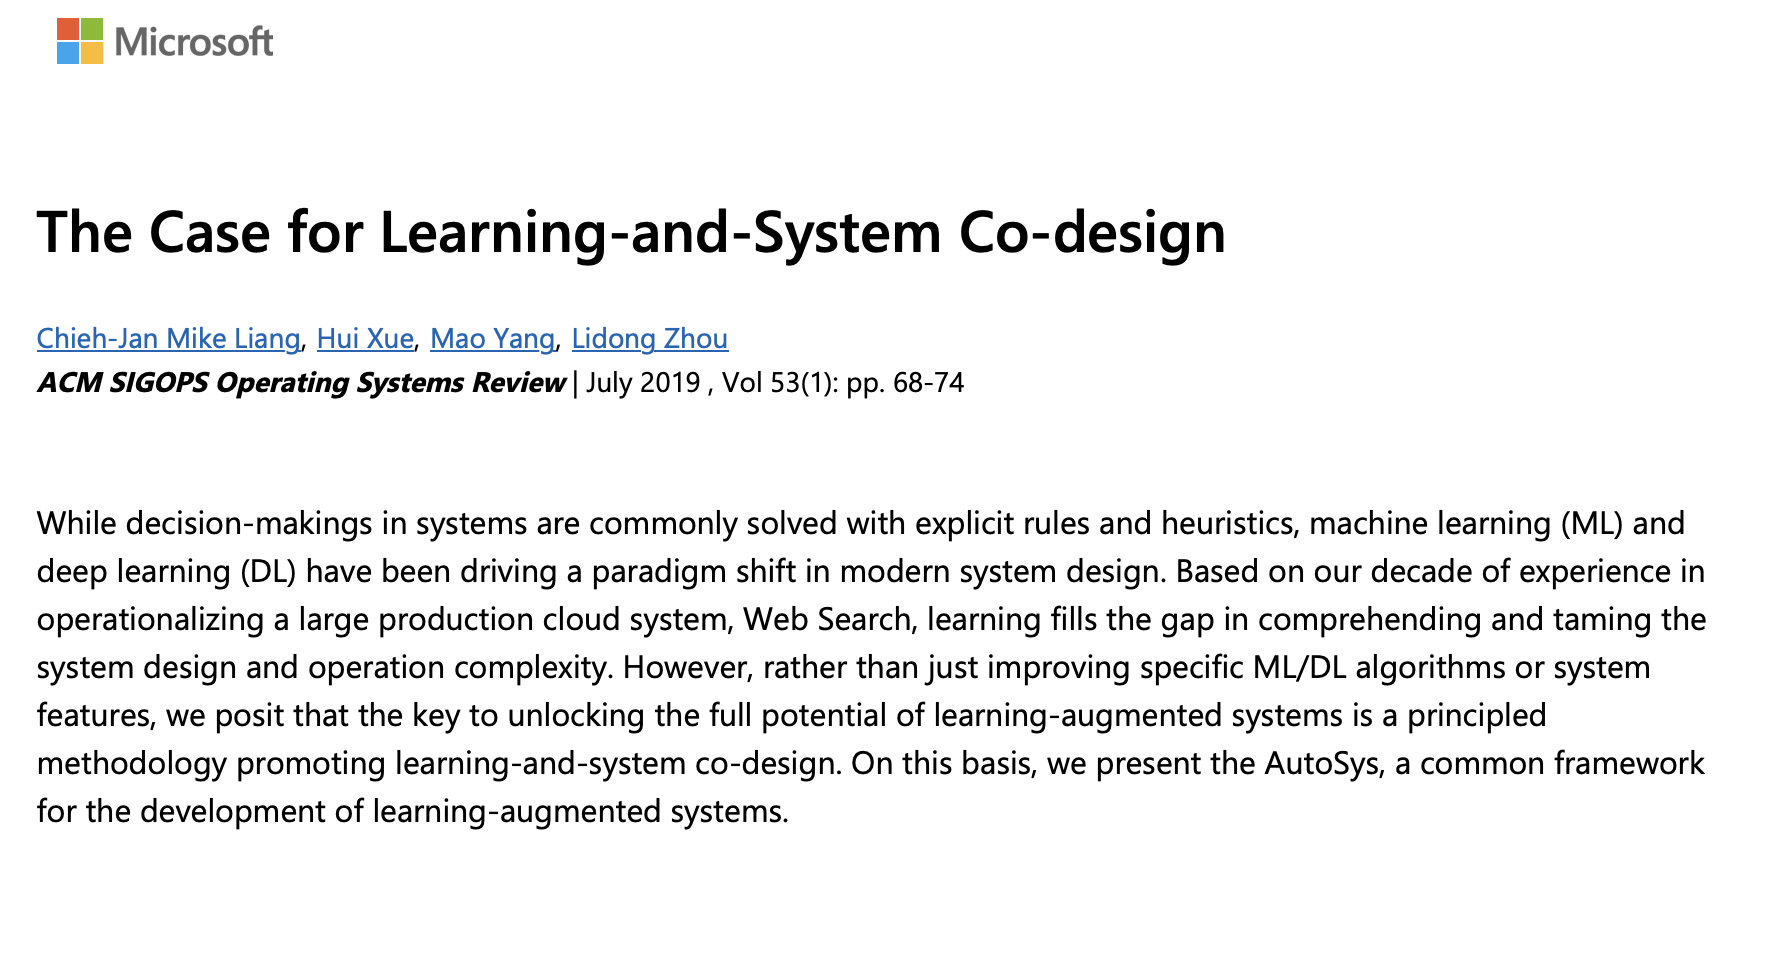
\includegraphics[height=180pt]{figure/co_design.png}
\end{frame}

\begin{frame}{Research}
  What is a good sys4ml/ml4sys research?
  \begin{itemize}
    \item<2-> Should be both good AI and systems research
      \begin{itemize}
        \item<3-> Provides insights to both communities
      \end{itemize}
    \item<4-> Leverages understanding of both domains
    \item<5-> I don't like adjust those parameters
  \end{itemize}
\end{frame}

\begin{frame}
  \Huge{\centerline{Thank you!}}
\end{frame}

\end{document}